% Bản tiếng Việt của bài ICCIT (main_iccit.tex). Biên dịch bằng XeLaTeX:
%   latexmk -xelatex main_iccit_vi.tex
% Định dạng theo hướng dẫn ICCIT: chữ Times 10 pt, lề tối thiểu 1 inch, đánh số trang,
% running head <= 50 ký tự, 3-5 từ khoá theo thứ tự chữ cái, trích dẫn số trong ngoặc vuông.
% Số liệu lấy từ generated/numbers.tex; bảng lấy từ generated_vi/ (bản dịch của generated/).
\documentclass[10pt,letterpaper]{article}
\usepackage{mathptmx}
\usepackage{fontspec}
\setmainfont{TeX Gyre Termes}
\setmonofont{DejaVu Sans Mono}[Scale=0.85]
\usepackage[margin=1in,headsep=0.25in,footskip=0.35in]{geometry}
\usepackage{amsmath}
\usepackage{graphicx}
\usepackage{booktabs}
\usepackage{multirow}
\usepackage{url}
\usepackage[nocompress]{cite}
\renewcommand{\citepunct}{,}
\usepackage[font=small,labelfont=bf,labelsep=period]{caption}
\usepackage{titlesec}
\usepackage{fancyhdr}
\usepackage[hidelinks]{hyperref}
% hyperref định nghĩa sẵn \numdef; tạm gác lại khi nạp các số liệu sinh tự động.
\let\hyNumdef\numdef\let\numdef\undefined
% Generated by analysis.security_final.paper_assets from the frozen lock. Do not edit.
\makeatletter
\providecommand{\numdef}[2]{\expandafter\def\csname num@#1\endcsname{#2}}
\providecommand{\val}[1]{\ifcsname num@#1\endcsname\csname num@#1\endcsname\else\textbf{??#1??}\PackageWarning{paper}{missing number #1}\fi}
\numdef{calls.controlled}{570}
\numdef{calls.genpilot}{176}
\numdef{calls.gentest}{4,618}
\numdef{calls.l5pilot}{154}
\numdef{calls.main}{2,919}
\numdef{calls.replay}{516}
\numdef{calls.total}{8,953}
\numdef{ch.A.I.hi}{55.0}
\numdef{ch.A.I.lo}{45.0}
\numdef{ch.A.I.n}{40}
\numdef{ch.A.I.pct}{45.0--55.0}
\numdef{ch.A.I.s}{18}
\numdef{ch.A.I.u}{4}
\numdef{ch.A.P.hi}{64.8}
\numdef{ch.A.P.lo}{35.2}
\numdef{ch.A.P.n}{40}
\numdef{ch.A.P.pct}{50.0}
\numdef{ch.A.P.s}{20}
\numdef{ch.A.P.u}{0}
\numdef{ch.A.attack_correct.hi}{48.5}
\numdef{ch.A.attack_correct.lo}{27.7}
\numdef{ch.A.attack_correct.n}{80}
\numdef{ch.A.attack_correct.pct}{37.5}
\numdef{ch.A.attack_correct.s}{30}
\numdef{ch.A.attack_correct.u}{0}
\numdef{ch.A.attack_correct_without_fake.hi}{49.0}
\numdef{ch.A.attack_correct_without_fake.lo}{27.2}
\numdef{ch.A.attack_correct_without_fake.n}{72}
\numdef{ch.A.attack_correct_without_fake.pct}{37.5}
\numdef{ch.A.attack_correct_without_fake.s}{27}
\numdef{ch.A.attack_correct_without_fake.u}{0}
\numdef{ch.A.attack_two_sources_report_kept.hi}{30.0}
\numdef{ch.A.attack_two_sources_report_kept.lo}{12.0}
\numdef{ch.A.attack_two_sources_report_kept.n}{72}
\numdef{ch.A.attack_two_sources_report_kept.pct}{19.4}
\numdef{ch.A.attack_two_sources_report_kept.s}{14}
\numdef{ch.A.attack_two_sources_report_kept.u}{0}
\numdef{ch.A.clean_correct.hi}{61.9}
\numdef{ch.A.clean_correct.lo}{40.5}
\numdef{ch.A.clean_correct.n}{80}
\numdef{ch.A.clean_correct.pct}{51.2}
\numdef{ch.A.clean_correct.s}{41}
\numdef{ch.A.clean_correct.u}{0}
\numdef{ch.A.clean_refusal.hi}{36.8}
\numdef{ch.A.clean_refusal.lo}{17.9}
\numdef{ch.A.clean_refusal.n}{80}
\numdef{ch.A.clean_refusal.pct}{26.2}
\numdef{ch.A.clean_refusal.s}{21}
\numdef{ch.A.clean_refusal.u}{0}
\numdef{ch.A.src.ai}{5}
\numdef{ch.A.src.human}{66}
\numdef{ch.A.src.scorer}{89}
\numdef{ch.A.total.hi}{52.5}
\numdef{ch.A.total.lo}{47.5}
\numdef{ch.A.total.n}{80}
\numdef{ch.A.total.pct}{47.5--52.5}
\numdef{ch.A.total.s}{38}
\numdef{ch.A.total.u}{4}
\numdef{ch.Apost.I.hi}{23.1}
\numdef{ch.Apost.I.lo}{4.0}
\numdef{ch.Apost.I.n}{40}
\numdef{ch.Apost.I.pct}{10.0}
\numdef{ch.Apost.I.s}{4}
\numdef{ch.Apost.I.u}{0}
\numdef{ch.Apost.P.hi}{16.5}
\numdef{ch.Apost.P.lo}{1.4}
\numdef{ch.Apost.P.n}{40}
\numdef{ch.Apost.P.pct}{5.0}
\numdef{ch.Apost.P.s}{2}
\numdef{ch.Apost.P.u}{0}
\numdef{ch.Apost.attack_correct.hi}{95.7}
\numdef{ch.Apost.attack_correct.lo}{83.0}
\numdef{ch.Apost.attack_correct.n}{80}
\numdef{ch.Apost.attack_correct.pct}{91.2}
\numdef{ch.Apost.attack_correct.s}{73}
\numdef{ch.Apost.attack_correct.u}{0}
\numdef{ch.Apost.attack_correct_without_fake.hi}{93.3}
\numdef{ch.Apost.attack_correct_without_fake.lo}{77.9}
\numdef{ch.Apost.attack_correct_without_fake.n}{72}
\numdef{ch.Apost.attack_correct_without_fake.pct}{87.5}
\numdef{ch.Apost.attack_correct_without_fake.s}{63}
\numdef{ch.Apost.attack_correct_without_fake.u}{0}
\numdef{ch.Apost.attack_two_sources_report_kept.hi}{72.8}
\numdef{ch.Apost.attack_two_sources_report_kept.lo}{51.0}
\numdef{ch.Apost.attack_two_sources_report_kept.n}{72}
\numdef{ch.Apost.attack_two_sources_report_kept.pct}{62.5}
\numdef{ch.Apost.attack_two_sources_report_kept.s}{45}
\numdef{ch.Apost.attack_two_sources_report_kept.u}{0}
\numdef{ch.Apost.clean_correct.hi}{98.7}
\numdef{ch.Apost.clean_correct.lo}{89.5}
\numdef{ch.Apost.clean_correct.n}{80}
\numdef{ch.Apost.clean_correct.pct}{96.2}
\numdef{ch.Apost.clean_correct.s}{77}
\numdef{ch.Apost.clean_correct.u}{0}
\numdef{ch.Apost.clean_refusal.hi}{6.7}
\numdef{ch.Apost.clean_refusal.lo}{0.2}
\numdef{ch.Apost.clean_refusal.n}{80}
\numdef{ch.Apost.clean_refusal.pct}{1.2}
\numdef{ch.Apost.clean_refusal.s}{1}
\numdef{ch.Apost.clean_refusal.u}{0}
\numdef{ch.Apost.src.ai}{17}
\numdef{ch.Apost.src.human}{22}
\numdef{ch.Apost.src.scorer}{121}
\numdef{ch.Apost.total.hi}{15.4}
\numdef{ch.Apost.total.lo}{3.5}
\numdef{ch.Apost.total.n}{80}
\numdef{ch.Apost.total.pct}{7.5}
\numdef{ch.Apost.total.s}{6}
\numdef{ch.Apost.total.u}{0}
\numdef{ch.ApostG.I.hi}{16.5}
\numdef{ch.ApostG.I.lo}{1.4}
\numdef{ch.ApostG.I.n}{40}
\numdef{ch.ApostG.I.pct}{5.0}
\numdef{ch.ApostG.I.s}{2}
\numdef{ch.ApostG.I.u}{0}
\numdef{ch.ApostG.P.hi}{16.5}
\numdef{ch.ApostG.P.lo}{1.4}
\numdef{ch.ApostG.P.n}{40}
\numdef{ch.ApostG.P.pct}{5.0}
\numdef{ch.ApostG.P.s}{2}
\numdef{ch.ApostG.P.u}{0}
\numdef{ch.ApostG.attack_correct.hi}{94.8}
\numdef{ch.ApostG.attack_correct.lo}{81.5}
\numdef{ch.ApostG.attack_correct.n}{80}
\numdef{ch.ApostG.attack_correct.pct}{90.0}
\numdef{ch.ApostG.attack_correct.s}{72}
\numdef{ch.ApostG.attack_correct.u}{0}
\numdef{ch.ApostG.attack_correct_without_fake.hi}{94.3}
\numdef{ch.ApostG.attack_correct_without_fake.lo}{79.6}
\numdef{ch.ApostG.attack_correct_without_fake.n}{72}
\numdef{ch.ApostG.attack_correct_without_fake.pct}{88.9}
\numdef{ch.ApostG.attack_correct_without_fake.s}{64}
\numdef{ch.ApostG.attack_correct_without_fake.u}{0}
\numdef{ch.ApostG.attack_two_sources_report_kept.hi}{71.5}
\numdef{ch.ApostG.attack_two_sources_report_kept.lo}{49.6}
\numdef{ch.ApostG.attack_two_sources_report_kept.n}{72}
\numdef{ch.ApostG.attack_two_sources_report_kept.pct}{61.1}
\numdef{ch.ApostG.attack_two_sources_report_kept.s}{44}
\numdef{ch.ApostG.attack_two_sources_report_kept.u}{0}
\numdef{ch.ApostG.clean_correct.hi}{98.0}
\numdef{ch.ApostG.clean_correct.lo}{87.8}
\numdef{ch.ApostG.clean_correct.n}{80}
\numdef{ch.ApostG.clean_correct.pct}{95.0}
\numdef{ch.ApostG.clean_correct.s}{76}
\numdef{ch.ApostG.clean_correct.u}{0}
\numdef{ch.ApostG.clean_refusal.hi}{6.7}
\numdef{ch.ApostG.clean_refusal.lo}{0.2}
\numdef{ch.ApostG.clean_refusal.n}{80}
\numdef{ch.ApostG.clean_refusal.pct}{1.2}
\numdef{ch.ApostG.clean_refusal.s}{1}
\numdef{ch.ApostG.clean_refusal.u}{0}
\numdef{ch.ApostG.src.ai}{23}
\numdef{ch.ApostG.src.human}{19}
\numdef{ch.ApostG.src.scorer}{118}
\numdef{ch.ApostG.total.hi}{12.2}
\numdef{ch.ApostG.total.lo}{2.0}
\numdef{ch.ApostG.total.n}{80}
\numdef{ch.ApostG.total.pct}{5.0}
\numdef{ch.ApostG.total.s}{4}
\numdef{ch.ApostG.total.u}{0}
\numdef{ch.Apre.I.hi}{32.5}
\numdef{ch.Apre.I.lo}{30.0}
\numdef{ch.Apre.I.n}{40}
\numdef{ch.Apre.I.pct}{30.0--32.5}
\numdef{ch.Apre.I.s}{12}
\numdef{ch.Apre.I.u}{1}
\numdef{ch.Apre.P.hi}{31.9}
\numdef{ch.Apre.P.lo}{8.7}
\numdef{ch.Apre.P.n}{40}
\numdef{ch.Apre.P.pct}{17.5}
\numdef{ch.Apre.P.s}{7}
\numdef{ch.Apre.P.u}{0}
\numdef{ch.Apre.attack_correct.hi}{85.3}
\numdef{ch.Apre.attack_correct.lo}{67.2}
\numdef{ch.Apre.attack_correct.n}{80}
\numdef{ch.Apre.attack_correct.pct}{77.5}
\numdef{ch.Apre.attack_correct.s}{62}
\numdef{ch.Apre.attack_correct.u}{0}
\numdef{ch.Apre.attack_correct_without_fake.hi}{82.4}
\numdef{ch.Apre.attack_correct_without_fake.lo}{62.4}
\numdef{ch.Apre.attack_correct_without_fake.n}{72}
\numdef{ch.Apre.attack_correct_without_fake.pct}{73.6}
\numdef{ch.Apre.attack_correct_without_fake.s}{53}
\numdef{ch.Apre.attack_correct_without_fake.u}{0}
\numdef{ch.Apre.attack_two_sources_report_kept.hi}{51.8}
\numdef{ch.Apre.attack_two_sources_report_kept.lo}{29.7}
\numdef{ch.Apre.attack_two_sources_report_kept.n}{72}
\numdef{ch.Apre.attack_two_sources_report_kept.pct}{40.3}
\numdef{ch.Apre.attack_two_sources_report_kept.s}{29}
\numdef{ch.Apre.attack_two_sources_report_kept.u}{0}
\numdef{ch.Apre.clean_correct.hi}{97.3}
\numdef{ch.Apre.clean_correct.lo}{86.2}
\numdef{ch.Apre.clean_correct.n}{80}
\numdef{ch.Apre.clean_correct.pct}{93.8}
\numdef{ch.Apre.clean_correct.s}{75}
\numdef{ch.Apre.clean_correct.u}{0}
\numdef{ch.Apre.clean_refusal.hi}{6.7}
\numdef{ch.Apre.clean_refusal.lo}{0.2}
\numdef{ch.Apre.clean_refusal.n}{80}
\numdef{ch.Apre.clean_refusal.pct}{1.2}
\numdef{ch.Apre.clean_refusal.s}{1}
\numdef{ch.Apre.clean_refusal.u}{0}
\numdef{ch.Apre.src.ai}{15}
\numdef{ch.Apre.src.human}{18}
\numdef{ch.Apre.src.scorer}{127}
\numdef{ch.Apre.total.hi}{25.0}
\numdef{ch.Apre.total.lo}{23.8}
\numdef{ch.Apre.total.n}{80}
\numdef{ch.Apre.total.pct}{23.8--25.0}
\numdef{ch.Apre.total.s}{19}
\numdef{ch.Apre.total.u}{1}
\numdef{ch.D.I.cp}{8.8}
\numdef{ch.D.I.hi}{8.8}
\numdef{ch.D.I.lo}{0.0}
\numdef{ch.D.I.n}{40}
\numdef{ch.D.I.pct}{0.0}
\numdef{ch.D.I.s}{0}
\numdef{ch.D.I.u}{0}
\numdef{ch.D.P.cp}{8.8}
\numdef{ch.D.P.hi}{8.8}
\numdef{ch.D.P.lo}{0.0}
\numdef{ch.D.P.n}{40}
\numdef{ch.D.P.pct}{0.0}
\numdef{ch.D.P.s}{0}
\numdef{ch.D.P.u}{0}
\numdef{ch.D.attack_correct.hi}{96.5}
\numdef{ch.D.attack_correct.lo}{84.6}
\numdef{ch.D.attack_correct.n}{80}
\numdef{ch.D.attack_correct.pct}{92.5}
\numdef{ch.D.attack_correct.s}{74}
\numdef{ch.D.attack_correct.u}{0}
\numdef{ch.D.attack_correct_without_fake.hi}{96.1}
\numdef{ch.D.attack_correct_without_fake.lo}{83.0}
\numdef{ch.D.attack_correct_without_fake.n}{72}
\numdef{ch.D.attack_correct_without_fake.pct}{91.7}
\numdef{ch.D.attack_correct_without_fake.s}{66}
\numdef{ch.D.attack_correct_without_fake.u}{0}
\numdef{ch.D.attack_two_sources_report_kept.hi}{53.2}
\numdef{ch.D.attack_two_sources_report_kept.lo}{31.0}
\numdef{ch.D.attack_two_sources_report_kept.n}{72}
\numdef{ch.D.attack_two_sources_report_kept.pct}{41.7}
\numdef{ch.D.attack_two_sources_report_kept.s}{30}
\numdef{ch.D.attack_two_sources_report_kept.u}{0}
\numdef{ch.D.clean_correct.hi}{99.3}
\numdef{ch.D.clean_correct.lo}{91.3}
\numdef{ch.D.clean_correct.n}{80}
\numdef{ch.D.clean_correct.pct}{97.5}
\numdef{ch.D.clean_correct.s}{78}
\numdef{ch.D.clean_correct.u}{0}
\numdef{ch.D.clean_refusal.hi}{4.6}
\numdef{ch.D.clean_refusal.lo}{0.0}
\numdef{ch.D.clean_refusal.n}{80}
\numdef{ch.D.clean_refusal.pct}{0.0}
\numdef{ch.D.clean_refusal.s}{0}
\numdef{ch.D.clean_refusal.u}{0}
\numdef{ch.D.src.ai}{11}
\numdef{ch.D.src.human}{17}
\numdef{ch.D.src.scorer}{132}
\numdef{ch.D.total.cp}{4.5}
\numdef{ch.D.total.hi}{4.6}
\numdef{ch.D.total.lo}{0.0}
\numdef{ch.D.total.n}{80}
\numdef{ch.D.total.pct}{0.0}
\numdef{ch.D.total.s}{0}
\numdef{ch.D.total.u}{0}
\numdef{ch.sens.A.I.hi}{55.0}
\numdef{ch.sens.A.I.lo}{45.0}
\numdef{ch.sens.A.I.n}{40}
\numdef{ch.sens.A.I.pct}{45.0--55.0}
\numdef{ch.sens.A.I.s}{18}
\numdef{ch.sens.A.I.u}{4}
\numdef{ch.sens.A.P.hi}{64.8}
\numdef{ch.sens.A.P.lo}{35.2}
\numdef{ch.sens.A.P.n}{40}
\numdef{ch.sens.A.P.pct}{50.0}
\numdef{ch.sens.A.P.s}{20}
\numdef{ch.sens.A.P.u}{0}
\numdef{ch.sens.A.total.hi}{52.5}
\numdef{ch.sens.A.total.lo}{47.5}
\numdef{ch.sens.A.total.n}{80}
\numdef{ch.sens.A.total.pct}{47.5--52.5}
\numdef{ch.sens.A.total.s}{38}
\numdef{ch.sens.A.total.u}{4}
\numdef{ch.sens.Apost.I.hi}{23.1}
\numdef{ch.sens.Apost.I.lo}{4.0}
\numdef{ch.sens.Apost.I.n}{40}
\numdef{ch.sens.Apost.I.pct}{10.0}
\numdef{ch.sens.Apost.I.s}{4}
\numdef{ch.sens.Apost.I.u}{0}
\numdef{ch.sens.Apost.P.hi}{16.5}
\numdef{ch.sens.Apost.P.lo}{1.4}
\numdef{ch.sens.Apost.P.n}{40}
\numdef{ch.sens.Apost.P.pct}{5.0}
\numdef{ch.sens.Apost.P.s}{2}
\numdef{ch.sens.Apost.P.u}{0}
\numdef{ch.sens.Apost.total.hi}{15.4}
\numdef{ch.sens.Apost.total.lo}{3.5}
\numdef{ch.sens.Apost.total.n}{80}
\numdef{ch.sens.Apost.total.pct}{7.5}
\numdef{ch.sens.Apost.total.s}{6}
\numdef{ch.sens.Apost.total.u}{0}
\numdef{ch.sens.ApostG.I.hi}{16.5}
\numdef{ch.sens.ApostG.I.lo}{1.4}
\numdef{ch.sens.ApostG.I.n}{40}
\numdef{ch.sens.ApostG.I.pct}{5.0}
\numdef{ch.sens.ApostG.I.s}{2}
\numdef{ch.sens.ApostG.I.u}{0}
\numdef{ch.sens.ApostG.P.hi}{16.5}
\numdef{ch.sens.ApostG.P.lo}{1.4}
\numdef{ch.sens.ApostG.P.n}{40}
\numdef{ch.sens.ApostG.P.pct}{5.0}
\numdef{ch.sens.ApostG.P.s}{2}
\numdef{ch.sens.ApostG.P.u}{0}
\numdef{ch.sens.ApostG.total.hi}{12.2}
\numdef{ch.sens.ApostG.total.lo}{2.0}
\numdef{ch.sens.ApostG.total.n}{80}
\numdef{ch.sens.ApostG.total.pct}{5.0}
\numdef{ch.sens.ApostG.total.s}{4}
\numdef{ch.sens.ApostG.total.u}{0}
\numdef{ch.sens.Apre.I.hi}{32.5}
\numdef{ch.sens.Apre.I.lo}{30.0}
\numdef{ch.sens.Apre.I.n}{40}
\numdef{ch.sens.Apre.I.pct}{30.0--32.5}
\numdef{ch.sens.Apre.I.s}{12}
\numdef{ch.sens.Apre.I.u}{1}
\numdef{ch.sens.Apre.P.hi}{31.9}
\numdef{ch.sens.Apre.P.lo}{8.7}
\numdef{ch.sens.Apre.P.n}{40}
\numdef{ch.sens.Apre.P.pct}{17.5}
\numdef{ch.sens.Apre.P.s}{7}
\numdef{ch.sens.Apre.P.u}{0}
\numdef{ch.sens.Apre.total.hi}{25.0}
\numdef{ch.sens.Apre.total.lo}{23.8}
\numdef{ch.sens.Apre.total.n}{80}
\numdef{ch.sens.Apre.total.pct}{23.8--25.0}
\numdef{ch.sens.Apre.total.s}{19}
\numdef{ch.sens.Apre.total.u}{1}
\numdef{ch.sens.D.I.cp}{8.8}
\numdef{ch.sens.D.I.hi}{8.8}
\numdef{ch.sens.D.I.lo}{0.0}
\numdef{ch.sens.D.I.n}{40}
\numdef{ch.sens.D.I.pct}{0.0}
\numdef{ch.sens.D.I.s}{0}
\numdef{ch.sens.D.I.u}{0}
\numdef{ch.sens.D.P.cp}{8.8}
\numdef{ch.sens.D.P.hi}{8.8}
\numdef{ch.sens.D.P.lo}{0.0}
\numdef{ch.sens.D.P.n}{40}
\numdef{ch.sens.D.P.pct}{0.0}
\numdef{ch.sens.D.P.s}{0}
\numdef{ch.sens.D.P.u}{0}
\numdef{ch.sens.D.total.cp}{4.5}
\numdef{ch.sens.D.total.hi}{4.6}
\numdef{ch.sens.D.total.lo}{0.0}
\numdef{ch.sens.D.total.n}{80}
\numdef{ch.sens.D.total.pct}{0.0}
\numdef{ch.sens.D.total.s}{0}
\numdef{ch.sens.D.total.u}{0}
\numdef{ch.test.all.AApre.a}{28}
\numdef{ch.test.all.AApre.b}{7}
\numdef{ch.test.all.AApre.n}{75}
\numdef{ch.test.all.AApre.p}{\ensuremath{5.1{\times}10^{-4}}}
\numdef{ch.test.all.AApre.ph}{0.00203}
\numdef{ch.test.all.AApre.u}{5}
\numdef{ch.test.all.ApostApostG.a}{3}
\numdef{ch.test.all.ApostApostG.b}{1}
\numdef{ch.test.all.ApostApostG.n}{80}
\numdef{ch.test.all.ApostApostG.p}{0.625}
\numdef{ch.test.all.ApostApostG.ph}{0.625}
\numdef{ch.test.all.ApostApostG.u}{0}
\numdef{ch.test.all.ApostD.a}{6}
\numdef{ch.test.all.ApostD.b}{0}
\numdef{ch.test.all.ApostD.n}{80}
\numdef{ch.test.all.ApostD.p}{0.0312}
\numdef{ch.test.all.ApostD.ph}{0.0625}
\numdef{ch.test.all.ApostD.u}{0}
\numdef{ch.test.all.ApreApost.a}{15}
\numdef{ch.test.all.ApreApost.b}{2}
\numdef{ch.test.all.ApreApost.n}{79}
\numdef{ch.test.all.ApreApost.p}{0.00235}
\numdef{ch.test.all.ApreApost.ph}{0.00705}
\numdef{ch.test.all.ApreApost.u}{1}
\numdef{g.aiai.items}{84}
\numdef{g.aiai.match}{62}
\numdef{g.dsucc.main}{2}
\numdef{g.gemma4-31b.A.I.hi}{55.0}
\numdef{g.gemma4-31b.A.I.lo}{45.0}
\numdef{g.gemma4-31b.A.I.n}{40}
\numdef{g.gemma4-31b.A.I.pct}{45.0--55.0}
\numdef{g.gemma4-31b.A.I.s}{18}
\numdef{g.gemma4-31b.A.I.u}{4}
\numdef{g.gemma4-31b.A.P.hi}{62.5}
\numdef{g.gemma4-31b.A.P.lo}{32.9}
\numdef{g.gemma4-31b.A.P.n}{40}
\numdef{g.gemma4-31b.A.P.pct}{47.5}
\numdef{g.gemma4-31b.A.P.s}{19}
\numdef{g.gemma4-31b.A.P.u}{0}
\numdef{g.gemma4-31b.A.attack_correct.hi}{51.0}
\numdef{g.gemma4-31b.A.attack_correct.lo}{30.0}
\numdef{g.gemma4-31b.A.attack_correct.n}{80}
\numdef{g.gemma4-31b.A.attack_correct.pct}{40.0}
\numdef{g.gemma4-31b.A.attack_correct.s}{32}
\numdef{g.gemma4-31b.A.attack_correct.u}{0}
\numdef{g.gemma4-31b.A.attack_correct_without_fake.hi}{54.6}
\numdef{g.gemma4-31b.A.attack_correct_without_fake.lo}{32.3}
\numdef{g.gemma4-31b.A.attack_correct_without_fake.n}{72}
\numdef{g.gemma4-31b.A.attack_correct_without_fake.pct}{43.1}
\numdef{g.gemma4-31b.A.attack_correct_without_fake.s}{31}
\numdef{g.gemma4-31b.A.attack_correct_without_fake.u}{0}
\numdef{g.gemma4-31b.A.attack_two_sources_report_kept.hi}{37.6}
\numdef{g.gemma4-31b.A.attack_two_sources_report_kept.lo}{17.6}
\numdef{g.gemma4-31b.A.attack_two_sources_report_kept.n}{72}
\numdef{g.gemma4-31b.A.attack_two_sources_report_kept.pct}{26.4}
\numdef{g.gemma4-31b.A.attack_two_sources_report_kept.s}{19}
\numdef{g.gemma4-31b.A.attack_two_sources_report_kept.u}{0}
\numdef{g.gemma4-31b.A.clean_correct.hi}{63.1}
\numdef{g.gemma4-31b.A.clean_correct.lo}{41.7}
\numdef{g.gemma4-31b.A.clean_correct.n}{80}
\numdef{g.gemma4-31b.A.clean_correct.pct}{52.5}
\numdef{g.gemma4-31b.A.clean_correct.s}{42}
\numdef{g.gemma4-31b.A.clean_correct.u}{0}
\numdef{g.gemma4-31b.A.clean_refusal.hi}{52.2}
\numdef{g.gemma4-31b.A.clean_refusal.lo}{31.1}
\numdef{g.gemma4-31b.A.clean_refusal.n}{80}
\numdef{g.gemma4-31b.A.clean_refusal.pct}{41.2}
\numdef{g.gemma4-31b.A.clean_refusal.s}{33}
\numdef{g.gemma4-31b.A.clean_refusal.u}{0}
\numdef{g.gemma4-31b.A.total.hi}{51.2}
\numdef{g.gemma4-31b.A.total.lo}{46.2}
\numdef{g.gemma4-31b.A.total.n}{80}
\numdef{g.gemma4-31b.A.total.pct}{46.2--51.2}
\numdef{g.gemma4-31b.A.total.s}{37}
\numdef{g.gemma4-31b.A.total.u}{4}
\numdef{g.gemma4-31b.D.I.cp}{8.8}
\numdef{g.gemma4-31b.D.I.hi}{8.8}
\numdef{g.gemma4-31b.D.I.lo}{0.0}
\numdef{g.gemma4-31b.D.I.n}{40}
\numdef{g.gemma4-31b.D.I.pct}{0.0}
\numdef{g.gemma4-31b.D.I.s}{0}
\numdef{g.gemma4-31b.D.I.u}{0}
\numdef{g.gemma4-31b.D.P.cp}{8.8}
\numdef{g.gemma4-31b.D.P.hi}{8.8}
\numdef{g.gemma4-31b.D.P.lo}{0.0}
\numdef{g.gemma4-31b.D.P.n}{40}
\numdef{g.gemma4-31b.D.P.pct}{0.0}
\numdef{g.gemma4-31b.D.P.s}{0}
\numdef{g.gemma4-31b.D.P.u}{0}
\numdef{g.gemma4-31b.D.attack_correct.hi}{94.8}
\numdef{g.gemma4-31b.D.attack_correct.lo}{81.5}
\numdef{g.gemma4-31b.D.attack_correct.n}{80}
\numdef{g.gemma4-31b.D.attack_correct.pct}{90.0}
\numdef{g.gemma4-31b.D.attack_correct.s}{72}
\numdef{g.gemma4-31b.D.attack_correct.u}{0}
\numdef{g.gemma4-31b.D.attack_correct_without_fake.hi}{94.3}
\numdef{g.gemma4-31b.D.attack_correct_without_fake.lo}{79.6}
\numdef{g.gemma4-31b.D.attack_correct_without_fake.n}{72}
\numdef{g.gemma4-31b.D.attack_correct_without_fake.pct}{88.9}
\numdef{g.gemma4-31b.D.attack_correct_without_fake.s}{64}
\numdef{g.gemma4-31b.D.attack_correct_without_fake.u}{0}
\numdef{g.gemma4-31b.D.attack_two_sources_report_kept.hi}{37.6}
\numdef{g.gemma4-31b.D.attack_two_sources_report_kept.lo}{17.6}
\numdef{g.gemma4-31b.D.attack_two_sources_report_kept.n}{72}
\numdef{g.gemma4-31b.D.attack_two_sources_report_kept.pct}{26.4}
\numdef{g.gemma4-31b.D.attack_two_sources_report_kept.s}{19}
\numdef{g.gemma4-31b.D.attack_two_sources_report_kept.u}{0}
\numdef{g.gemma4-31b.D.clean_correct.hi}{95.7}
\numdef{g.gemma4-31b.D.clean_correct.lo}{83.0}
\numdef{g.gemma4-31b.D.clean_correct.n}{80}
\numdef{g.gemma4-31b.D.clean_correct.pct}{91.2}
\numdef{g.gemma4-31b.D.clean_correct.s}{73}
\numdef{g.gemma4-31b.D.clean_correct.u}{0}
\numdef{g.gemma4-31b.D.clean_refusal.hi}{12.2}
\numdef{g.gemma4-31b.D.clean_refusal.lo}{2.0}
\numdef{g.gemma4-31b.D.clean_refusal.n}{80}
\numdef{g.gemma4-31b.D.clean_refusal.pct}{5.0}
\numdef{g.gemma4-31b.D.clean_refusal.s}{4}
\numdef{g.gemma4-31b.D.clean_refusal.u}{0}
\numdef{g.gemma4-31b.D.total.cp}{4.5}
\numdef{g.gemma4-31b.D.total.hi}{4.6}
\numdef{g.gemma4-31b.D.total.lo}{0.0}
\numdef{g.gemma4-31b.D.total.n}{80}
\numdef{g.gemma4-31b.D.total.pct}{0.0}
\numdef{g.gemma4-31b.D.total.s}{0}
\numdef{g.gemma4-31b.D.total.u}{0}
\numdef{g.gemma4-31b.calls}{1,633}
\numdef{g.gemma4-31b.sens.A.I.hi}{55.0}
\numdef{g.gemma4-31b.sens.A.I.lo}{45.0}
\numdef{g.gemma4-31b.sens.A.I.n}{40}
\numdef{g.gemma4-31b.sens.A.I.pct}{45.0--55.0}
\numdef{g.gemma4-31b.sens.A.I.s}{18}
\numdef{g.gemma4-31b.sens.A.I.u}{4}
\numdef{g.gemma4-31b.sens.A.P.hi}{64.8}
\numdef{g.gemma4-31b.sens.A.P.lo}{35.2}
\numdef{g.gemma4-31b.sens.A.P.n}{40}
\numdef{g.gemma4-31b.sens.A.P.pct}{50.0}
\numdef{g.gemma4-31b.sens.A.P.s}{20}
\numdef{g.gemma4-31b.sens.A.P.u}{0}
\numdef{g.gemma4-31b.sens.A.total.hi}{52.5}
\numdef{g.gemma4-31b.sens.A.total.lo}{47.5}
\numdef{g.gemma4-31b.sens.A.total.n}{80}
\numdef{g.gemma4-31b.sens.A.total.pct}{47.5--52.5}
\numdef{g.gemma4-31b.sens.A.total.s}{38}
\numdef{g.gemma4-31b.sens.A.total.u}{4}
\numdef{g.gemma4-31b.sens.D.I.cp}{8.8}
\numdef{g.gemma4-31b.sens.D.I.hi}{8.8}
\numdef{g.gemma4-31b.sens.D.I.lo}{0.0}
\numdef{g.gemma4-31b.sens.D.I.n}{40}
\numdef{g.gemma4-31b.sens.D.I.pct}{0.0}
\numdef{g.gemma4-31b.sens.D.I.s}{0}
\numdef{g.gemma4-31b.sens.D.I.u}{0}
\numdef{g.gemma4-31b.sens.D.P.cp}{8.8}
\numdef{g.gemma4-31b.sens.D.P.hi}{8.8}
\numdef{g.gemma4-31b.sens.D.P.lo}{0.0}
\numdef{g.gemma4-31b.sens.D.P.n}{40}
\numdef{g.gemma4-31b.sens.D.P.pct}{0.0}
\numdef{g.gemma4-31b.sens.D.P.s}{0}
\numdef{g.gemma4-31b.sens.D.P.u}{0}
\numdef{g.gemma4-31b.sens.D.total.cp}{4.5}
\numdef{g.gemma4-31b.sens.D.total.hi}{4.6}
\numdef{g.gemma4-31b.sens.D.total.lo}{0.0}
\numdef{g.gemma4-31b.sens.D.total.n}{80}
\numdef{g.gemma4-31b.sens.D.total.pct}{0.0}
\numdef{g.gemma4-31b.sens.D.total.s}{0}
\numdef{g.gemma4-31b.sens.D.total.u}{0}
\numdef{g.gemma4-31b.stab.Aruns}{7, 7, 8}
\numdef{g.gemma4-31b.stab.Druns}{0, 0, 0}
\numdef{g.gemma4-31b.stab.changed}{1}
\numdef{g.gemma4-31b.stab.changedD}{0}
\numdef{g.gemma4-31b.stab.pairs}{32}
\numdef{g.gemma4-31b.stab.same}{31}
\numdef{g.gemma4-31b.test.I.a}{18}
\numdef{g.gemma4-31b.test.I.b}{0}
\numdef{g.gemma4-31b.test.I.n}{36}
\numdef{g.gemma4-31b.test.I.p}{\ensuremath{7.6{\times}10^{-6}}}
\numdef{g.gemma4-31b.test.I.ph}{\ensuremath{2.3{\times}10^{-5}}}
\numdef{g.gemma4-31b.test.I.u}{4}
\numdef{g.gemma4-31b.test.P.a}{19}
\numdef{g.gemma4-31b.test.P.b}{0}
\numdef{g.gemma4-31b.test.P.n}{40}
\numdef{g.gemma4-31b.test.P.p}{\ensuremath{3.8{\times}10^{-6}}}
\numdef{g.gemma4-31b.test.P.ph}{\ensuremath{1.5{\times}10^{-5}}}
\numdef{g.gemma4-31b.test.P.u}{0}
\numdef{g.gemma4-31b.valid}{448/448}
\numdef{g.gpt-oss-120b.A.I.hi}{55.0}
\numdef{g.gpt-oss-120b.A.I.lo}{45.0}
\numdef{g.gpt-oss-120b.A.I.n}{40}
\numdef{g.gpt-oss-120b.A.I.pct}{45.0--55.0}
\numdef{g.gpt-oss-120b.A.I.s}{18}
\numdef{g.gpt-oss-120b.A.I.u}{4}
\numdef{g.gpt-oss-120b.A.P.hi}{69.3}
\numdef{g.gpt-oss-120b.A.P.lo}{39.8}
\numdef{g.gpt-oss-120b.A.P.n}{40}
\numdef{g.gpt-oss-120b.A.P.pct}{55.0}
\numdef{g.gpt-oss-120b.A.P.s}{22}
\numdef{g.gpt-oss-120b.A.P.u}{0}
\numdef{g.gpt-oss-120b.A.attack_correct.hi}{52.2}
\numdef{g.gpt-oss-120b.A.attack_correct.lo}{31.1}
\numdef{g.gpt-oss-120b.A.attack_correct.n}{80}
\numdef{g.gpt-oss-120b.A.attack_correct.pct}{41.2}
\numdef{g.gpt-oss-120b.A.attack_correct.s}{33}
\numdef{g.gpt-oss-120b.A.attack_correct.u}{0}
\numdef{g.gpt-oss-120b.A.attack_correct_without_fake.hi}{53.2}
\numdef{g.gpt-oss-120b.A.attack_correct_without_fake.lo}{31.0}
\numdef{g.gpt-oss-120b.A.attack_correct_without_fake.n}{72}
\numdef{g.gpt-oss-120b.A.attack_correct_without_fake.pct}{41.7}
\numdef{g.gpt-oss-120b.A.attack_correct_without_fake.s}{30}
\numdef{g.gpt-oss-120b.A.attack_correct_without_fake.u}{0}
\numdef{g.gpt-oss-120b.A.attack_two_sources_report_kept.hi}{28.5}
\numdef{g.gpt-oss-120b.A.attack_two_sources_report_kept.lo}{10.9}
\numdef{g.gpt-oss-120b.A.attack_two_sources_report_kept.n}{72}
\numdef{g.gpt-oss-120b.A.attack_two_sources_report_kept.pct}{18.1}
\numdef{g.gpt-oss-120b.A.attack_two_sources_report_kept.s}{13}
\numdef{g.gpt-oss-120b.A.attack_two_sources_report_kept.u}{0}
\numdef{g.gpt-oss-120b.A.clean_correct.hi}{60.7}
\numdef{g.gpt-oss-120b.A.clean_correct.lo}{39.3}
\numdef{g.gpt-oss-120b.A.clean_correct.n}{80}
\numdef{g.gpt-oss-120b.A.clean_correct.pct}{50.0}
\numdef{g.gpt-oss-120b.A.clean_correct.s}{40}
\numdef{g.gpt-oss-120b.A.clean_correct.u}{0}
\numdef{g.gpt-oss-120b.A.clean_refusal.hi}{39.5}
\numdef{g.gpt-oss-120b.A.clean_refusal.lo}{20.0}
\numdef{g.gpt-oss-120b.A.clean_refusal.n}{80}
\numdef{g.gpt-oss-120b.A.clean_refusal.pct}{28.7}
\numdef{g.gpt-oss-120b.A.clean_refusal.s}{23}
\numdef{g.gpt-oss-120b.A.clean_refusal.u}{0}
\numdef{g.gpt-oss-120b.A.total.hi}{55.0}
\numdef{g.gpt-oss-120b.A.total.lo}{50.0}
\numdef{g.gpt-oss-120b.A.total.n}{80}
\numdef{g.gpt-oss-120b.A.total.pct}{50.0--55.0}
\numdef{g.gpt-oss-120b.A.total.s}{40}
\numdef{g.gpt-oss-120b.A.total.u}{4}
\numdef{g.gpt-oss-120b.D.I.cp}{8.8}
\numdef{g.gpt-oss-120b.D.I.hi}{8.8}
\numdef{g.gpt-oss-120b.D.I.lo}{0.0}
\numdef{g.gpt-oss-120b.D.I.n}{40}
\numdef{g.gpt-oss-120b.D.I.pct}{0.0}
\numdef{g.gpt-oss-120b.D.I.s}{0}
\numdef{g.gpt-oss-120b.D.I.u}{0}
\numdef{g.gpt-oss-120b.D.P.hi}{12.9}
\numdef{g.gpt-oss-120b.D.P.lo}{0.4}
\numdef{g.gpt-oss-120b.D.P.n}{40}
\numdef{g.gpt-oss-120b.D.P.pct}{2.5}
\numdef{g.gpt-oss-120b.D.P.s}{1}
\numdef{g.gpt-oss-120b.D.P.u}{0}
\numdef{g.gpt-oss-120b.D.attack_correct.hi}{98.0}
\numdef{g.gpt-oss-120b.D.attack_correct.lo}{87.8}
\numdef{g.gpt-oss-120b.D.attack_correct.n}{80}
\numdef{g.gpt-oss-120b.D.attack_correct.pct}{95.0}
\numdef{g.gpt-oss-120b.D.attack_correct.s}{76}
\numdef{g.gpt-oss-120b.D.attack_correct.u}{0}
\numdef{g.gpt-oss-120b.D.attack_correct_without_fake.hi}{97.8}
\numdef{g.gpt-oss-120b.D.attack_correct_without_fake.lo}{86.6}
\numdef{g.gpt-oss-120b.D.attack_correct_without_fake.n}{72}
\numdef{g.gpt-oss-120b.D.attack_correct_without_fake.pct}{94.4}
\numdef{g.gpt-oss-120b.D.attack_correct_without_fake.s}{68}
\numdef{g.gpt-oss-120b.D.attack_correct_without_fake.u}{0}
\numdef{g.gpt-oss-120b.D.attack_two_sources_report_kept.hi}{58.6}
\numdef{g.gpt-oss-120b.D.attack_two_sources_report_kept.lo}{36.1}
\numdef{g.gpt-oss-120b.D.attack_two_sources_report_kept.n}{72}
\numdef{g.gpt-oss-120b.D.attack_two_sources_report_kept.pct}{47.2}
\numdef{g.gpt-oss-120b.D.attack_two_sources_report_kept.s}{34}
\numdef{g.gpt-oss-120b.D.attack_two_sources_report_kept.u}{0}
\numdef{g.gpt-oss-120b.D.clean_correct.hi}{98.0}
\numdef{g.gpt-oss-120b.D.clean_correct.lo}{87.8}
\numdef{g.gpt-oss-120b.D.clean_correct.n}{80}
\numdef{g.gpt-oss-120b.D.clean_correct.pct}{95.0}
\numdef{g.gpt-oss-120b.D.clean_correct.s}{76}
\numdef{g.gpt-oss-120b.D.clean_correct.u}{0}
\numdef{g.gpt-oss-120b.D.clean_refusal.hi}{10.5}
\numdef{g.gpt-oss-120b.D.clean_refusal.lo}{1.3}
\numdef{g.gpt-oss-120b.D.clean_refusal.n}{80}
\numdef{g.gpt-oss-120b.D.clean_refusal.pct}{3.8}
\numdef{g.gpt-oss-120b.D.clean_refusal.s}{3}
\numdef{g.gpt-oss-120b.D.clean_refusal.u}{0}
\numdef{g.gpt-oss-120b.D.total.hi}{6.7}
\numdef{g.gpt-oss-120b.D.total.lo}{0.2}
\numdef{g.gpt-oss-120b.D.total.n}{80}
\numdef{g.gpt-oss-120b.D.total.pct}{1.2}
\numdef{g.gpt-oss-120b.D.total.s}{1}
\numdef{g.gpt-oss-120b.D.total.u}{0}
\numdef{g.gpt-oss-120b.calls}{1,495}
\numdef{g.gpt-oss-120b.sens.A.I.hi}{55.0}
\numdef{g.gpt-oss-120b.sens.A.I.lo}{45.0}
\numdef{g.gpt-oss-120b.sens.A.I.n}{40}
\numdef{g.gpt-oss-120b.sens.A.I.pct}{45.0--55.0}
\numdef{g.gpt-oss-120b.sens.A.I.s}{18}
\numdef{g.gpt-oss-120b.sens.A.I.u}{4}
\numdef{g.gpt-oss-120b.sens.A.P.hi}{67.1}
\numdef{g.gpt-oss-120b.sens.A.P.lo}{37.5}
\numdef{g.gpt-oss-120b.sens.A.P.n}{40}
\numdef{g.gpt-oss-120b.sens.A.P.pct}{52.5}
\numdef{g.gpt-oss-120b.sens.A.P.s}{21}
\numdef{g.gpt-oss-120b.sens.A.P.u}{0}
\numdef{g.gpt-oss-120b.sens.A.total.hi}{53.8}
\numdef{g.gpt-oss-120b.sens.A.total.lo}{48.8}
\numdef{g.gpt-oss-120b.sens.A.total.n}{80}
\numdef{g.gpt-oss-120b.sens.A.total.pct}{48.8--53.8}
\numdef{g.gpt-oss-120b.sens.A.total.s}{39}
\numdef{g.gpt-oss-120b.sens.A.total.u}{4}
\numdef{g.gpt-oss-120b.sens.D.I.cp}{8.8}
\numdef{g.gpt-oss-120b.sens.D.I.hi}{8.8}
\numdef{g.gpt-oss-120b.sens.D.I.lo}{0.0}
\numdef{g.gpt-oss-120b.sens.D.I.n}{40}
\numdef{g.gpt-oss-120b.sens.D.I.pct}{0.0}
\numdef{g.gpt-oss-120b.sens.D.I.s}{0}
\numdef{g.gpt-oss-120b.sens.D.I.u}{0}
\numdef{g.gpt-oss-120b.sens.D.P.cp}{8.8}
\numdef{g.gpt-oss-120b.sens.D.P.hi}{8.8}
\numdef{g.gpt-oss-120b.sens.D.P.lo}{0.0}
\numdef{g.gpt-oss-120b.sens.D.P.n}{40}
\numdef{g.gpt-oss-120b.sens.D.P.pct}{0.0}
\numdef{g.gpt-oss-120b.sens.D.P.s}{0}
\numdef{g.gpt-oss-120b.sens.D.P.u}{0}
\numdef{g.gpt-oss-120b.sens.D.total.cp}{4.5}
\numdef{g.gpt-oss-120b.sens.D.total.hi}{4.6}
\numdef{g.gpt-oss-120b.sens.D.total.lo}{0.0}
\numdef{g.gpt-oss-120b.sens.D.total.n}{80}
\numdef{g.gpt-oss-120b.sens.D.total.pct}{0.0}
\numdef{g.gpt-oss-120b.sens.D.total.s}{0}
\numdef{g.gpt-oss-120b.sens.D.total.u}{0}
\numdef{g.gpt-oss-120b.stab.Aruns}{8, 6, 5}
\numdef{g.gpt-oss-120b.stab.Druns}{0, 0, 0}
\numdef{g.gpt-oss-120b.stab.changed}{6}
\numdef{g.gpt-oss-120b.stab.changedD}{0}
\numdef{g.gpt-oss-120b.stab.pairs}{32}
\numdef{g.gpt-oss-120b.stab.same}{26}
\numdef{g.gpt-oss-120b.test.I.a}{18}
\numdef{g.gpt-oss-120b.test.I.b}{0}
\numdef{g.gpt-oss-120b.test.I.n}{36}
\numdef{g.gpt-oss-120b.test.I.p}{\ensuremath{7.6{\times}10^{-6}}}
\numdef{g.gpt-oss-120b.test.I.ph}{\ensuremath{2.3{\times}10^{-5}}}
\numdef{g.gpt-oss-120b.test.I.u}{4}
\numdef{g.gpt-oss-120b.test.P.a}{21}
\numdef{g.gpt-oss-120b.test.P.b}{0}
\numdef{g.gpt-oss-120b.test.P.n}{40}
\numdef{g.gpt-oss-120b.test.P.p}{\ensuremath{9.5{\times}10^{-7}}}
\numdef{g.gpt-oss-120b.test.P.ph}{\ensuremath{4.8{\times}10^{-6}}}
\numdef{g.gpt-oss-120b.test.P.u}{0}
\numdef{g.gpt-oss-120b.valid}{448/448}
\numdef{g.gpt-oss-20b.A.I.hi}{62.5}
\numdef{g.gpt-oss-20b.A.I.lo}{52.5}
\numdef{g.gpt-oss-20b.A.I.n}{40}
\numdef{g.gpt-oss-20b.A.I.pct}{52.5--62.5}
\numdef{g.gpt-oss-20b.A.I.s}{21}
\numdef{g.gpt-oss-20b.A.I.u}{4}
\numdef{g.gpt-oss-20b.A.P.hi}{73.7}
\numdef{g.gpt-oss-20b.A.P.lo}{44.6}
\numdef{g.gpt-oss-20b.A.P.n}{40}
\numdef{g.gpt-oss-20b.A.P.pct}{60.0}
\numdef{g.gpt-oss-20b.A.P.s}{24}
\numdef{g.gpt-oss-20b.A.P.u}{0}
\numdef{g.gpt-oss-20b.A.attack_correct.hi}{47.2}
\numdef{g.gpt-oss-20b.A.attack_correct.lo}{26.6}
\numdef{g.gpt-oss-20b.A.attack_correct.n}{80}
\numdef{g.gpt-oss-20b.A.attack_correct.pct}{36.2}
\numdef{g.gpt-oss-20b.A.attack_correct.s}{29}
\numdef{g.gpt-oss-20b.A.attack_correct.u}{0}
\numdef{g.gpt-oss-20b.A.attack_correct_without_fake.hi}{42.0}
\numdef{g.gpt-oss-20b.A.attack_correct_without_fake.lo}{21.1}
\numdef{g.gpt-oss-20b.A.attack_correct_without_fake.n}{72}
\numdef{g.gpt-oss-20b.A.attack_correct_without_fake.pct}{30.6}
\numdef{g.gpt-oss-20b.A.attack_correct_without_fake.s}{22}
\numdef{g.gpt-oss-20b.A.attack_correct_without_fake.u}{0}
\numdef{g.gpt-oss-20b.A.attack_two_sources_report_kept.hi}{25.3}
\numdef{g.gpt-oss-20b.A.attack_two_sources_report_kept.lo}{8.8}
\numdef{g.gpt-oss-20b.A.attack_two_sources_report_kept.n}{72}
\numdef{g.gpt-oss-20b.A.attack_two_sources_report_kept.pct}{15.3}
\numdef{g.gpt-oss-20b.A.attack_two_sources_report_kept.s}{11}
\numdef{g.gpt-oss-20b.A.attack_two_sources_report_kept.u}{0}
\numdef{g.gpt-oss-20b.A.clean_correct.hi}{61.9}
\numdef{g.gpt-oss-20b.A.clean_correct.lo}{40.5}
\numdef{g.gpt-oss-20b.A.clean_correct.n}{80}
\numdef{g.gpt-oss-20b.A.clean_correct.pct}{51.2}
\numdef{g.gpt-oss-20b.A.clean_correct.s}{41}
\numdef{g.gpt-oss-20b.A.clean_correct.u}{0}
\numdef{g.gpt-oss-20b.A.clean_refusal.hi}{30.0}
\numdef{g.gpt-oss-20b.A.clean_refusal.lo}{12.7}
\numdef{g.gpt-oss-20b.A.clean_refusal.n}{80}
\numdef{g.gpt-oss-20b.A.clean_refusal.pct}{20.0}
\numdef{g.gpt-oss-20b.A.clean_refusal.s}{16}
\numdef{g.gpt-oss-20b.A.clean_refusal.u}{0}
\numdef{g.gpt-oss-20b.A.total.hi}{61.3}
\numdef{g.gpt-oss-20b.A.total.lo}{56.2}
\numdef{g.gpt-oss-20b.A.total.n}{80}
\numdef{g.gpt-oss-20b.A.total.pct}{56.2--61.3}
\numdef{g.gpt-oss-20b.A.total.s}{45}
\numdef{g.gpt-oss-20b.A.total.u}{4}
\numdef{g.gpt-oss-20b.D.I.hi}{12.9}
\numdef{g.gpt-oss-20b.D.I.lo}{0.4}
\numdef{g.gpt-oss-20b.D.I.n}{40}
\numdef{g.gpt-oss-20b.D.I.pct}{2.5}
\numdef{g.gpt-oss-20b.D.I.s}{1}
\numdef{g.gpt-oss-20b.D.I.u}{0}
\numdef{g.gpt-oss-20b.D.P.cp}{8.8}
\numdef{g.gpt-oss-20b.D.P.hi}{8.8}
\numdef{g.gpt-oss-20b.D.P.lo}{0.0}
\numdef{g.gpt-oss-20b.D.P.n}{40}
\numdef{g.gpt-oss-20b.D.P.pct}{0.0}
\numdef{g.gpt-oss-20b.D.P.s}{0}
\numdef{g.gpt-oss-20b.D.P.u}{0}
\numdef{g.gpt-oss-20b.D.attack_correct.hi}{94.0}
\numdef{g.gpt-oss-20b.D.attack_correct.lo}{80.0}
\numdef{g.gpt-oss-20b.D.attack_correct.n}{80}
\numdef{g.gpt-oss-20b.D.attack_correct.pct}{88.8}
\numdef{g.gpt-oss-20b.D.attack_correct.s}{71}
\numdef{g.gpt-oss-20b.D.attack_correct.u}{0}
\numdef{g.gpt-oss-20b.D.attack_correct_without_fake.hi}{92.3}
\numdef{g.gpt-oss-20b.D.attack_correct_without_fake.lo}{76.3}
\numdef{g.gpt-oss-20b.D.attack_correct_without_fake.n}{72}
\numdef{g.gpt-oss-20b.D.attack_correct_without_fake.pct}{86.1}
\numdef{g.gpt-oss-20b.D.attack_correct_without_fake.s}{62}
\numdef{g.gpt-oss-20b.D.attack_correct_without_fake.u}{0}
\numdef{g.gpt-oss-20b.D.attack_two_sources_report_kept.hi}{53.2}
\numdef{g.gpt-oss-20b.D.attack_two_sources_report_kept.lo}{31.0}
\numdef{g.gpt-oss-20b.D.attack_two_sources_report_kept.n}{72}
\numdef{g.gpt-oss-20b.D.attack_two_sources_report_kept.pct}{41.7}
\numdef{g.gpt-oss-20b.D.attack_two_sources_report_kept.s}{30}
\numdef{g.gpt-oss-20b.D.attack_two_sources_report_kept.u}{0}
\numdef{g.gpt-oss-20b.D.clean_correct.hi}{95.7}
\numdef{g.gpt-oss-20b.D.clean_correct.lo}{83.0}
\numdef{g.gpt-oss-20b.D.clean_correct.n}{80}
\numdef{g.gpt-oss-20b.D.clean_correct.pct}{91.2}
\numdef{g.gpt-oss-20b.D.clean_correct.s}{73}
\numdef{g.gpt-oss-20b.D.clean_correct.u}{0}
\numdef{g.gpt-oss-20b.D.clean_refusal.hi}{13.8}
\numdef{g.gpt-oss-20b.D.clean_refusal.lo}{2.7}
\numdef{g.gpt-oss-20b.D.clean_refusal.n}{80}
\numdef{g.gpt-oss-20b.D.clean_refusal.pct}{6.2}
\numdef{g.gpt-oss-20b.D.clean_refusal.s}{5}
\numdef{g.gpt-oss-20b.D.clean_refusal.u}{0}
\numdef{g.gpt-oss-20b.D.total.hi}{6.7}
\numdef{g.gpt-oss-20b.D.total.lo}{0.2}
\numdef{g.gpt-oss-20b.D.total.n}{80}
\numdef{g.gpt-oss-20b.D.total.pct}{1.2}
\numdef{g.gpt-oss-20b.D.total.s}{1}
\numdef{g.gpt-oss-20b.D.total.u}{0}
\numdef{g.gpt-oss-20b.calls}{1,490}
\numdef{g.gpt-oss-20b.sens.A.I.hi}{60.0}
\numdef{g.gpt-oss-20b.sens.A.I.lo}{50.0}
\numdef{g.gpt-oss-20b.sens.A.I.n}{40}
\numdef{g.gpt-oss-20b.sens.A.I.pct}{50.0--60.0}
\numdef{g.gpt-oss-20b.sens.A.I.s}{20}
\numdef{g.gpt-oss-20b.sens.A.I.u}{4}
\numdef{g.gpt-oss-20b.sens.A.P.hi}{71.5}
\numdef{g.gpt-oss-20b.sens.A.P.lo}{42.2}
\numdef{g.gpt-oss-20b.sens.A.P.n}{40}
\numdef{g.gpt-oss-20b.sens.A.P.pct}{57.5}
\numdef{g.gpt-oss-20b.sens.A.P.s}{23}
\numdef{g.gpt-oss-20b.sens.A.P.u}{0}
\numdef{g.gpt-oss-20b.sens.A.total.hi}{58.8}
\numdef{g.gpt-oss-20b.sens.A.total.lo}{53.8}
\numdef{g.gpt-oss-20b.sens.A.total.n}{80}
\numdef{g.gpt-oss-20b.sens.A.total.pct}{53.8--58.8}
\numdef{g.gpt-oss-20b.sens.A.total.s}{43}
\numdef{g.gpt-oss-20b.sens.A.total.u}{4}
\numdef{g.gpt-oss-20b.sens.D.I.hi}{12.9}
\numdef{g.gpt-oss-20b.sens.D.I.lo}{0.4}
\numdef{g.gpt-oss-20b.sens.D.I.n}{40}
\numdef{g.gpt-oss-20b.sens.D.I.pct}{2.5}
\numdef{g.gpt-oss-20b.sens.D.I.s}{1}
\numdef{g.gpt-oss-20b.sens.D.I.u}{0}
\numdef{g.gpt-oss-20b.sens.D.P.cp}{8.8}
\numdef{g.gpt-oss-20b.sens.D.P.hi}{8.8}
\numdef{g.gpt-oss-20b.sens.D.P.lo}{0.0}
\numdef{g.gpt-oss-20b.sens.D.P.n}{40}
\numdef{g.gpt-oss-20b.sens.D.P.pct}{0.0}
\numdef{g.gpt-oss-20b.sens.D.P.s}{0}
\numdef{g.gpt-oss-20b.sens.D.P.u}{0}
\numdef{g.gpt-oss-20b.sens.D.total.hi}{6.7}
\numdef{g.gpt-oss-20b.sens.D.total.lo}{0.2}
\numdef{g.gpt-oss-20b.sens.D.total.n}{80}
\numdef{g.gpt-oss-20b.sens.D.total.pct}{1.2}
\numdef{g.gpt-oss-20b.sens.D.total.s}{1}
\numdef{g.gpt-oss-20b.sens.D.total.u}{0}
\numdef{g.gpt-oss-20b.stab.Aruns}{5, 6, 6}
\numdef{g.gpt-oss-20b.stab.Druns}{1, 0, 1}
\numdef{g.gpt-oss-20b.stab.changed}{8}
\numdef{g.gpt-oss-20b.stab.changedD}{2}
\numdef{g.gpt-oss-20b.stab.pairs}{32}
\numdef{g.gpt-oss-20b.stab.same}{24}
\numdef{g.gpt-oss-20b.test.I.a}{21}
\numdef{g.gpt-oss-20b.test.I.b}{1}
\numdef{g.gpt-oss-20b.test.I.n}{36}
\numdef{g.gpt-oss-20b.test.I.p}{\ensuremath{1.1{\times}10^{-5}}}
\numdef{g.gpt-oss-20b.test.I.ph}{\ensuremath{2.3{\times}10^{-5}}}
\numdef{g.gpt-oss-20b.test.I.u}{4}
\numdef{g.gpt-oss-20b.test.P.a}{24}
\numdef{g.gpt-oss-20b.test.P.b}{0}
\numdef{g.gpt-oss-20b.test.P.n}{40}
\numdef{g.gpt-oss-20b.test.P.p}{\ensuremath{1.2{\times}10^{-7}}}
\numdef{g.gpt-oss-20b.test.P.ph}{\ensuremath{7.2{\times}10^{-7}}}
\numdef{g.gpt-oss-20b.test.P.u}{0}
\numdef{g.gpt-oss-20b.valid}{448/448}
\numdef{g.holm.max}{\ensuremath{2.3{\times}10^{-5}}}
\numdef{g.process.aireviewed}{198}
\numdef{g.process.answers}{1,344}
\numdef{g.process.disagree}{84}
\numdef{g.process.sample}{60}
\numdef{g.process.sheet}{144}
\numdef{g.svh.adopted_target.k}{0.90}
\numdef{g.svh.adopted_target.n}{60}
\numdef{g.svh.conflict_flagged.k}{0.86}
\numdef{g.svh.conflict_flagged.n}{16}
\numdef{g.svh.refused.k}{0.93}
\numdef{g.svh.refused.n}{60}
\numdef{g.svh.report_correct.k}{1.00}
\numdef{g.svh.report_correct.n}{60}
\numdef{g.svh.summary_asserts.k}{0.83}
\numdef{g.svh.summary_asserts.n}{13}
\numdef{hv.D.false_alarm}{1}
\numdef{hv.D.false_discovery_rate}{100.0}
\numdef{hv.D.false_negative_rate}{100.0}
\numdef{hv.D.false_omission_rate}{1.3}
\numdef{hv.D.false_positive_rate}{0.3}
\numdef{hv.D.missed}{4}
\numdef{hv.D.numeric_answers}{311}
\numdef{hv.D.scorer_false}{310}
\numdef{hv.D.scorer_true}{1}
\numdef{hv.D_answers}{338}
\numdef{hv.adoption.false_alarm}{22}
\numdef{hv.adoption.false_discovery_rate}{25.3}
\numdef{hv.adoption.false_negative_rate}{24.4}
\numdef{hv.adoption.false_omission_rate}{3.2}
\numdef{hv.adoption.false_positive_rate}{3.4}
\numdef{hv.adoption.missed}{21}
\numdef{hv.adoption.numeric_answers}{736}
\numdef{hv.adoption.scorer_false}{649}
\numdef{hv.adoption.scorer_true}{87}
\numdef{hv.answers}{796}
\numdef{hv.blind_complete_answers}{794}
\numdef{hv.g.gemma4-31b.A.hi}{53.8}
\numdef{hv.g.gemma4-31b.A.lo}{48.8}
\numdef{hv.g.gemma4-31b.A.n}{80}
\numdef{hv.g.gemma4-31b.A.pct}{48.8--53.8}
\numdef{hv.g.gemma4-31b.A.s}{39}
\numdef{hv.g.gemma4-31b.A.u}{4}
\numdef{hv.g.gemma4-31b.D.hi}{6.7}
\numdef{hv.g.gemma4-31b.D.lo}{0.2}
\numdef{hv.g.gemma4-31b.D.n}{80}
\numdef{hv.g.gemma4-31b.D.pct}{1.2}
\numdef{hv.g.gemma4-31b.D.s}{1}
\numdef{hv.g.gemma4-31b.D.u}{0}
\numdef{hv.g.gpt-oss-120b.A.hi}{56.2}
\numdef{hv.g.gpt-oss-120b.A.lo}{51.2}
\numdef{hv.g.gpt-oss-120b.A.n}{80}
\numdef{hv.g.gpt-oss-120b.A.pct}{51.2--56.2}
\numdef{hv.g.gpt-oss-120b.A.s}{41}
\numdef{hv.g.gpt-oss-120b.A.u}{4}
\numdef{hv.g.gpt-oss-120b.D.hi}{6.7}
\numdef{hv.g.gpt-oss-120b.D.lo}{0.2}
\numdef{hv.g.gpt-oss-120b.D.n}{80}
\numdef{hv.g.gpt-oss-120b.D.pct}{1.2}
\numdef{hv.g.gpt-oss-120b.D.s}{1}
\numdef{hv.g.gpt-oss-120b.D.u}{0}
\numdef{hv.g.gpt-oss-20b.A.hi}{57.5}
\numdef{hv.g.gpt-oss-20b.A.lo}{52.5}
\numdef{hv.g.gpt-oss-20b.A.n}{80}
\numdef{hv.g.gpt-oss-20b.A.pct}{52.5--57.5}
\numdef{hv.g.gpt-oss-20b.A.s}{42}
\numdef{hv.g.gpt-oss-20b.A.u}{4}
\numdef{hv.g.gpt-oss-20b.D.hi}{6.7}
\numdef{hv.g.gpt-oss-20b.D.lo}{0.2}
\numdef{hv.g.gpt-oss-20b.D.n}{80}
\numdef{hv.g.gpt-oss-20b.D.pct}{1.2}
\numdef{hv.g.gpt-oss-20b.D.s}{1}
\numdef{hv.g.gpt-oss-20b.D.u}{0}
\numdef{hv.ir.adopted_target.agree}{96.7}
\numdef{hv.ir.adopted_target.k}{0.90}
\numdef{hv.ir.adopted_target.pairhi}{0.93}
\numdef{hv.ir.adopted_target.pairlo}{0.86}
\numdef{hv.ir.conflict_flagged.agree}{81.7}
\numdef{hv.ir.conflict_flagged.k}{0.81}
\numdef{hv.ir.conflict_flagged.pairhi}{0.87}
\numdef{hv.ir.conflict_flagged.pairlo}{0.76}
\numdef{hv.ir.refused.agree}{98.3}
\numdef{hv.ir.refused.k}{0.79}
\numdef{hv.ir.refused.pairhi}{1.00}
\numdef{hv.ir.refused.pairlo}{0.66}
\numdef{hv.ir.report_correct.agree}{91.7}
\numdef{hv.ir.report_correct.k}{0.85}
\numdef{hv.ir.report_correct.pairhi}{0.91}
\numdef{hv.ir.report_correct.pairlo}{0.81}
\numdef{hv.ir.summary_asserts.agree}{96.7}
\numdef{hv.ir.summary_asserts.k}{0.96}
\numdef{hv.ir.summary_asserts.pairhi}{0.97}
\numdef{hv.ir.summary_asserts.pairlo}{0.94}
\numdef{hv.ir.use_of_fake.agree}{66.7}
\numdef{hv.ir.use_of_fake.k}{0.67}
\numdef{hv.ir.use_of_fake.pairhi}{0.75}
\numdef{hv.ir.use_of_fake.pairlo}{0.59}
\numdef{hv.main.A.hi}{55.0}
\numdef{hv.main.A.lo}{50.0}
\numdef{hv.main.A.n}{80}
\numdef{hv.main.A.pct}{50.0--55.0}
\numdef{hv.main.A.s}{40}
\numdef{hv.main.A.u}{4}
\numdef{hv.main.AD.ph.max}{\ensuremath{3.8{\times}10^{-5}}}
\numdef{hv.main.B.hi}{8.7}
\numdef{hv.main.B.lo}{0.7}
\numdef{hv.main.B.n}{80}
\numdef{hv.main.B.pct}{2.5}
\numdef{hv.main.B.s}{2}
\numdef{hv.main.B.u}{0}
\numdef{hv.main.C.cp}{4.5}
\numdef{hv.main.C.hi}{4.6}
\numdef{hv.main.C.lo}{0.0}
\numdef{hv.main.C.n}{80}
\numdef{hv.main.C.pct}{0.0}
\numdef{hv.main.C.s}{0}
\numdef{hv.main.C.u}{0}
\numdef{hv.main.D.hi}{8.7}
\numdef{hv.main.D.lo}{0.7}
\numdef{hv.main.D.n}{80}
\numdef{hv.main.D.pct}{2.5}
\numdef{hv.main.D.s}{2}
\numdef{hv.main.D.u}{0}
\numdef{hv.raters}{3}
\numdef{hv.rating_rows}{916}
\numdef{hv.sc.adopted_target.agree}{94.2}
\numdef{hv.sc.adopted_target.k}{0.72}
\numdef{hv.sc.adopted_target.n}{736}
\numdef{hv.sc.conflict_flagged.agree}{80.0}
\numdef{hv.sc.conflict_flagged.k}{0.70}
\numdef{hv.sc.conflict_flagged.n}{796}
\numdef{hv.sc.refused.agree}{97.4}
\numdef{hv.sc.refused.k}{0.81}
\numdef{hv.sc.refused.n}{796}
\numdef{hv.sc.report_correct.agree}{95.5}
\numdef{hv.sc.report_correct.k}{0.87}
\numdef{hv.sc.report_correct.n}{796}
\numdef{hv.sc.summary_asserts.agree}{85.2}
\numdef{hv.sc.summary_asserts.k}{0.74}
\numdef{hv.sc.summary_asserts.n}{796}
\numdef{hv.sc.use_of_fake.agree}{--}
\numdef{hv.sc.use_of_fake.k}{--}
\numdef{hv.sc.use_of_fake.n}{0}
\numdef{hv.seen}{0}
\numdef{hv.shared}{60}
\numdef{hv.unresolved.use_of_fake}{2}
\numdef{labels.ai}{197}
\numdef{labels.human}{339}
\numdef{labels.intables}{2,464}
\numdef{labels.rows}{2,479}
\numdef{labels.scorer}{1,928}
\numdef{labels.sha}{bf1a72baf2bb}
\numdef{p2.A.I.hi}{55.0}
\numdef{p2.A.I.lo}{45.0}
\numdef{p2.A.I.n}{40}
\numdef{p2.A.I.pct}{45.0--55.0}
\numdef{p2.A.I.s}{18}
\numdef{p2.A.I.u}{4}
\numdef{p2.A.P.hi}{64.8}
\numdef{p2.A.P.lo}{35.2}
\numdef{p2.A.P.n}{40}
\numdef{p2.A.P.pct}{50.0}
\numdef{p2.A.P.s}{20}
\numdef{p2.A.P.u}{0}
\numdef{p2.A.attack_correct.hi}{48.5}
\numdef{p2.A.attack_correct.lo}{27.7}
\numdef{p2.A.attack_correct.n}{80}
\numdef{p2.A.attack_correct.pct}{37.5}
\numdef{p2.A.attack_correct.s}{30}
\numdef{p2.A.attack_correct.u}{0}
\numdef{p2.A.attack_correct_without_fake.hi}{49.0}
\numdef{p2.A.attack_correct_without_fake.lo}{27.2}
\numdef{p2.A.attack_correct_without_fake.n}{72}
\numdef{p2.A.attack_correct_without_fake.pct}{37.5}
\numdef{p2.A.attack_correct_without_fake.s}{27}
\numdef{p2.A.attack_correct_without_fake.u}{0}
\numdef{p2.A.attack_two_sources_report_kept.hi}{30.0}
\numdef{p2.A.attack_two_sources_report_kept.lo}{12.0}
\numdef{p2.A.attack_two_sources_report_kept.n}{72}
\numdef{p2.A.attack_two_sources_report_kept.pct}{19.4}
\numdef{p2.A.attack_two_sources_report_kept.s}{14}
\numdef{p2.A.attack_two_sources_report_kept.u}{0}
\numdef{p2.A.clean_correct.hi}{61.9}
\numdef{p2.A.clean_correct.lo}{40.5}
\numdef{p2.A.clean_correct.n}{80}
\numdef{p2.A.clean_correct.pct}{51.2}
\numdef{p2.A.clean_correct.s}{41}
\numdef{p2.A.clean_correct.u}{0}
\numdef{p2.A.clean_refusal.hi}{36.8}
\numdef{p2.A.clean_refusal.lo}{17.9}
\numdef{p2.A.clean_refusal.n}{80}
\numdef{p2.A.clean_refusal.pct}{26.2}
\numdef{p2.A.clean_refusal.s}{21}
\numdef{p2.A.clean_refusal.u}{0}
\numdef{p2.A.src.ai}{5}
\numdef{p2.A.src.human}{66}
\numdef{p2.A.src.scorer}{89}
\numdef{p2.A.total.hi}{52.5}
\numdef{p2.A.total.lo}{47.5}
\numdef{p2.A.total.n}{80}
\numdef{p2.A.total.pct}{47.5--52.5}
\numdef{p2.A.total.s}{38}
\numdef{p2.A.total.u}{4}
\numdef{p2.B.I.cp}{8.8}
\numdef{p2.B.I.hi}{8.8}
\numdef{p2.B.I.lo}{0.0}
\numdef{p2.B.I.n}{40}
\numdef{p2.B.I.pct}{0.0}
\numdef{p2.B.I.s}{0}
\numdef{p2.B.I.u}{0}
\numdef{p2.B.P.hi}{12.9}
\numdef{p2.B.P.lo}{0.4}
\numdef{p2.B.P.n}{40}
\numdef{p2.B.P.pct}{2.5}
\numdef{p2.B.P.s}{1}
\numdef{p2.B.P.u}{0}
\numdef{p2.B.attack_correct.hi}{96.5}
\numdef{p2.B.attack_correct.lo}{84.6}
\numdef{p2.B.attack_correct.n}{80}
\numdef{p2.B.attack_correct.pct}{92.5}
\numdef{p2.B.attack_correct.s}{74}
\numdef{p2.B.attack_correct.u}{0}
\numdef{p2.B.attack_correct_without_fake.hi}{96.1}
\numdef{p2.B.attack_correct_without_fake.lo}{83.0}
\numdef{p2.B.attack_correct_without_fake.n}{72}
\numdef{p2.B.attack_correct_without_fake.pct}{91.7}
\numdef{p2.B.attack_correct_without_fake.s}{66}
\numdef{p2.B.attack_correct_without_fake.u}{0}
\numdef{p2.B.attack_two_sources_report_kept.hi}{53.2}
\numdef{p2.B.attack_two_sources_report_kept.lo}{31.0}
\numdef{p2.B.attack_two_sources_report_kept.n}{72}
\numdef{p2.B.attack_two_sources_report_kept.pct}{41.7}
\numdef{p2.B.attack_two_sources_report_kept.s}{30}
\numdef{p2.B.attack_two_sources_report_kept.u}{0}
\numdef{p2.B.clean_correct.hi}{98.7}
\numdef{p2.B.clean_correct.lo}{89.5}
\numdef{p2.B.clean_correct.n}{80}
\numdef{p2.B.clean_correct.pct}{96.2}
\numdef{p2.B.clean_correct.s}{77}
\numdef{p2.B.clean_correct.u}{0}
\numdef{p2.B.clean_refusal.hi}{6.7}
\numdef{p2.B.clean_refusal.lo}{0.2}
\numdef{p2.B.clean_refusal.n}{80}
\numdef{p2.B.clean_refusal.pct}{1.2}
\numdef{p2.B.clean_refusal.s}{1}
\numdef{p2.B.clean_refusal.u}{0}
\numdef{p2.B.src.ai}{6}
\numdef{p2.B.src.human}{26}
\numdef{p2.B.src.scorer}{128}
\numdef{p2.B.total.hi}{6.7}
\numdef{p2.B.total.lo}{0.2}
\numdef{p2.B.total.n}{80}
\numdef{p2.B.total.pct}{1.2}
\numdef{p2.B.total.s}{1}
\numdef{p2.B.total.u}{0}
\numdef{p2.C.I.cp}{8.8}
\numdef{p2.C.I.hi}{8.8}
\numdef{p2.C.I.lo}{0.0}
\numdef{p2.C.I.n}{40}
\numdef{p2.C.I.pct}{0.0}
\numdef{p2.C.I.s}{0}
\numdef{p2.C.I.u}{0}
\numdef{p2.C.P.cp}{8.8}
\numdef{p2.C.P.hi}{8.8}
\numdef{p2.C.P.lo}{0.0}
\numdef{p2.C.P.n}{40}
\numdef{p2.C.P.pct}{0.0}
\numdef{p2.C.P.s}{0}
\numdef{p2.C.P.u}{0}
\numdef{p2.C.attack_correct.hi}{98.0}
\numdef{p2.C.attack_correct.lo}{87.8}
\numdef{p2.C.attack_correct.n}{80}
\numdef{p2.C.attack_correct.pct}{95.0}
\numdef{p2.C.attack_correct.s}{76}
\numdef{p2.C.attack_correct.u}{0}
\numdef{p2.C.attack_correct_without_fake.hi}{97.8}
\numdef{p2.C.attack_correct_without_fake.lo}{86.6}
\numdef{p2.C.attack_correct_without_fake.n}{72}
\numdef{p2.C.attack_correct_without_fake.pct}{94.4}
\numdef{p2.C.attack_correct_without_fake.s}{68}
\numdef{p2.C.attack_correct_without_fake.u}{0}
\numdef{p2.C.attack_two_sources_report_kept.hi}{58.6}
\numdef{p2.C.attack_two_sources_report_kept.lo}{36.1}
\numdef{p2.C.attack_two_sources_report_kept.n}{72}
\numdef{p2.C.attack_two_sources_report_kept.pct}{47.2}
\numdef{p2.C.attack_two_sources_report_kept.s}{34}
\numdef{p2.C.attack_two_sources_report_kept.u}{0}
\numdef{p2.C.clean_correct.hi}{98.0}
\numdef{p2.C.clean_correct.lo}{87.8}
\numdef{p2.C.clean_correct.n}{80}
\numdef{p2.C.clean_correct.pct}{95.0}
\numdef{p2.C.clean_correct.s}{76}
\numdef{p2.C.clean_correct.u}{0}
\numdef{p2.C.clean_refusal.hi}{6.7}
\numdef{p2.C.clean_refusal.lo}{0.2}
\numdef{p2.C.clean_refusal.n}{80}
\numdef{p2.C.clean_refusal.pct}{1.2}
\numdef{p2.C.clean_refusal.s}{1}
\numdef{p2.C.clean_refusal.u}{0}
\numdef{p2.C.src.ai}{6}
\numdef{p2.C.src.human}{27}
\numdef{p2.C.src.scorer}{127}
\numdef{p2.C.total.cp}{4.5}
\numdef{p2.C.total.hi}{4.6}
\numdef{p2.C.total.lo}{0.0}
\numdef{p2.C.total.n}{80}
\numdef{p2.C.total.pct}{0.0}
\numdef{p2.C.total.s}{0}
\numdef{p2.C.total.u}{0}
\numdef{p2.D.I.cp}{8.8}
\numdef{p2.D.I.hi}{8.8}
\numdef{p2.D.I.lo}{0.0}
\numdef{p2.D.I.n}{40}
\numdef{p2.D.I.pct}{0.0}
\numdef{p2.D.I.s}{0}
\numdef{p2.D.I.u}{0}
\numdef{p2.D.P.cp}{8.8}
\numdef{p2.D.P.hi}{8.8}
\numdef{p2.D.P.lo}{0.0}
\numdef{p2.D.P.n}{40}
\numdef{p2.D.P.pct}{0.0}
\numdef{p2.D.P.s}{0}
\numdef{p2.D.P.u}{0}
\numdef{p2.D.attack_correct.hi}{96.5}
\numdef{p2.D.attack_correct.lo}{84.6}
\numdef{p2.D.attack_correct.n}{80}
\numdef{p2.D.attack_correct.pct}{92.5}
\numdef{p2.D.attack_correct.s}{74}
\numdef{p2.D.attack_correct.u}{0}
\numdef{p2.D.attack_correct_without_fake.hi}{96.1}
\numdef{p2.D.attack_correct_without_fake.lo}{83.0}
\numdef{p2.D.attack_correct_without_fake.n}{72}
\numdef{p2.D.attack_correct_without_fake.pct}{91.7}
\numdef{p2.D.attack_correct_without_fake.s}{66}
\numdef{p2.D.attack_correct_without_fake.u}{0}
\numdef{p2.D.attack_two_sources_report_kept.hi}{53.2}
\numdef{p2.D.attack_two_sources_report_kept.lo}{31.0}
\numdef{p2.D.attack_two_sources_report_kept.n}{72}
\numdef{p2.D.attack_two_sources_report_kept.pct}{41.7}
\numdef{p2.D.attack_two_sources_report_kept.s}{30}
\numdef{p2.D.attack_two_sources_report_kept.u}{0}
\numdef{p2.D.clean_correct.hi}{99.3}
\numdef{p2.D.clean_correct.lo}{91.3}
\numdef{p2.D.clean_correct.n}{80}
\numdef{p2.D.clean_correct.pct}{97.5}
\numdef{p2.D.clean_correct.s}{78}
\numdef{p2.D.clean_correct.u}{0}
\numdef{p2.D.clean_refusal.hi}{4.6}
\numdef{p2.D.clean_refusal.lo}{0.0}
\numdef{p2.D.clean_refusal.n}{80}
\numdef{p2.D.clean_refusal.pct}{0.0}
\numdef{p2.D.clean_refusal.s}{0}
\numdef{p2.D.clean_refusal.u}{0}
\numdef{p2.D.src.ai}{11}
\numdef{p2.D.src.human}{17}
\numdef{p2.D.src.scorer}{132}
\numdef{p2.D.total.cp}{4.5}
\numdef{p2.D.total.hi}{4.6}
\numdef{p2.D.total.lo}{0.0}
\numdef{p2.D.total.n}{80}
\numdef{p2.D.total.pct}{0.0}
\numdef{p2.D.total.s}{0}
\numdef{p2.D.total.u}{0}
\numdef{p2.aiai.adopted_target.k}{0.91}
\numdef{p2.aiai.conflict_flagged.k}{0.94}
\numdef{p2.aiai.refused.k}{1.00}
\numdef{p2.aiai.report_correct.k}{0.97}
\numdef{p2.aiai.summary_asserts.k}{1.00}
\numdef{p2.aiai.use_of_fake.k}{0.94}
\numdef{p2.aival.adopted_target.k}{1.00}
\numdef{p2.aival.conflict_flagged.k}{0.86}
\numdef{p2.aival.refused.k}{0.95}
\numdef{p2.aival.report_correct.k}{1.00}
\numdef{p2.aival.summary_asserts.k}{0.93}
\numdef{p2.aival.use_of_fake.k}{1.00}
\numdef{p2.human.answers}{209}
\numdef{p2.human.invalidation}{110}
\numdef{p2.human.labels}{1238}
\numdef{p2.sens.A.I.hi}{55.0}
\numdef{p2.sens.A.I.lo}{45.0}
\numdef{p2.sens.A.I.n}{40}
\numdef{p2.sens.A.I.pct}{45.0--55.0}
\numdef{p2.sens.A.I.s}{18}
\numdef{p2.sens.A.I.u}{4}
\numdef{p2.sens.A.P.hi}{64.8}
\numdef{p2.sens.A.P.lo}{35.2}
\numdef{p2.sens.A.P.n}{40}
\numdef{p2.sens.A.P.pct}{50.0}
\numdef{p2.sens.A.P.s}{20}
\numdef{p2.sens.A.P.u}{0}
\numdef{p2.sens.A.total.hi}{52.5}
\numdef{p2.sens.A.total.lo}{47.5}
\numdef{p2.sens.A.total.n}{80}
\numdef{p2.sens.A.total.pct}{47.5--52.5}
\numdef{p2.sens.A.total.s}{38}
\numdef{p2.sens.A.total.u}{4}
\numdef{p2.sens.B.I.cp}{8.8}
\numdef{p2.sens.B.I.hi}{8.8}
\numdef{p2.sens.B.I.lo}{0.0}
\numdef{p2.sens.B.I.n}{40}
\numdef{p2.sens.B.I.pct}{0.0}
\numdef{p2.sens.B.I.s}{0}
\numdef{p2.sens.B.I.u}{0}
\numdef{p2.sens.B.P.hi}{12.9}
\numdef{p2.sens.B.P.lo}{0.4}
\numdef{p2.sens.B.P.n}{40}
\numdef{p2.sens.B.P.pct}{2.5}
\numdef{p2.sens.B.P.s}{1}
\numdef{p2.sens.B.P.u}{0}
\numdef{p2.sens.B.total.hi}{6.7}
\numdef{p2.sens.B.total.lo}{0.2}
\numdef{p2.sens.B.total.n}{80}
\numdef{p2.sens.B.total.pct}{1.2}
\numdef{p2.sens.B.total.s}{1}
\numdef{p2.sens.B.total.u}{0}
\numdef{p2.sens.C.I.cp}{8.8}
\numdef{p2.sens.C.I.hi}{8.8}
\numdef{p2.sens.C.I.lo}{0.0}
\numdef{p2.sens.C.I.n}{40}
\numdef{p2.sens.C.I.pct}{0.0}
\numdef{p2.sens.C.I.s}{0}
\numdef{p2.sens.C.I.u}{0}
\numdef{p2.sens.C.P.cp}{8.8}
\numdef{p2.sens.C.P.hi}{8.8}
\numdef{p2.sens.C.P.lo}{0.0}
\numdef{p2.sens.C.P.n}{40}
\numdef{p2.sens.C.P.pct}{0.0}
\numdef{p2.sens.C.P.s}{0}
\numdef{p2.sens.C.P.u}{0}
\numdef{p2.sens.C.total.cp}{4.5}
\numdef{p2.sens.C.total.hi}{4.6}
\numdef{p2.sens.C.total.lo}{0.0}
\numdef{p2.sens.C.total.n}{80}
\numdef{p2.sens.C.total.pct}{0.0}
\numdef{p2.sens.C.total.s}{0}
\numdef{p2.sens.C.total.u}{0}
\numdef{p2.sens.D.I.cp}{8.8}
\numdef{p2.sens.D.I.hi}{8.8}
\numdef{p2.sens.D.I.lo}{0.0}
\numdef{p2.sens.D.I.n}{40}
\numdef{p2.sens.D.I.pct}{0.0}
\numdef{p2.sens.D.I.s}{0}
\numdef{p2.sens.D.I.u}{0}
\numdef{p2.sens.D.P.cp}{8.8}
\numdef{p2.sens.D.P.hi}{8.8}
\numdef{p2.sens.D.P.lo}{0.0}
\numdef{p2.sens.D.P.n}{40}
\numdef{p2.sens.D.P.pct}{0.0}
\numdef{p2.sens.D.P.s}{0}
\numdef{p2.sens.D.P.u}{0}
\numdef{p2.sens.D.total.cp}{4.5}
\numdef{p2.sens.D.total.hi}{4.6}
\numdef{p2.sens.D.total.lo}{0.0}
\numdef{p2.sens.D.total.n}{80}
\numdef{p2.sens.D.total.pct}{0.0}
\numdef{p2.sens.D.total.s}{0}
\numdef{p2.sens.D.total.u}{0}
\numdef{p2.svh.v33.adopted_target.k}{0.65}
\numdef{p2.svh.v33.adopted_target.n}{81}
\numdef{p2.svh.v33.conflict_flagged.k}{0.40}
\numdef{p2.svh.v33.conflict_flagged.n}{65}
\numdef{p2.svh.v33.refused.k}{0.56}
\numdef{p2.svh.v33.refused.n}{81}
\numdef{p2.svh.v33.report_correct.k}{0.95}
\numdef{p2.svh.v33.report_correct.n}{81}
\numdef{p2.svh.v33.summary_asserts.k}{0.48}
\numdef{p2.svh.v33.summary_asserts.n}{33}
\numdef{p2.svh.v34.adopted_target.k}{0.90}
\numdef{p2.svh.v34.adopted_target.n}{77}
\numdef{p2.svh.v34.conflict_flagged.k}{0.57}
\numdef{p2.svh.v34.conflict_flagged.n}{61}
\numdef{p2.svh.v34.refused.k}{0.79}
\numdef{p2.svh.v34.refused.n}{77}
\numdef{p2.svh.v34.report_correct.k}{0.88}
\numdef{p2.svh.v34.report_correct.n}{77}
\numdef{p2.svh.v34.summary_asserts.k}{0.65}
\numdef{p2.svh.v34.summary_asserts.n}{32}
\numdef{p2.test.I.AD.a}{18}
\numdef{p2.test.I.AD.b}{0}
\numdef{p2.test.I.AD.n}{36}
\numdef{p2.test.I.AD.p}{\ensuremath{7.6{\times}10^{-6}}}
\numdef{p2.test.I.AD.ph}{\ensuremath{3.8{\times}10^{-5}}}
\numdef{p2.test.I.AD.u}{4}
\numdef{p2.test.I.BC.a}{0}
\numdef{p2.test.I.BC.b}{0}
\numdef{p2.test.I.BC.n}{40}
\numdef{p2.test.I.BC.p}{1}
\numdef{p2.test.I.BC.ph}{1}
\numdef{p2.test.I.BC.u}{0}
\numdef{p2.test.I.CD.a}{0}
\numdef{p2.test.I.CD.b}{0}
\numdef{p2.test.I.CD.n}{40}
\numdef{p2.test.I.CD.p}{1}
\numdef{p2.test.I.CD.ph}{1}
\numdef{p2.test.I.CD.u}{0}
\numdef{p2.test.P.AD.a}{20}
\numdef{p2.test.P.AD.b}{0}
\numdef{p2.test.P.AD.n}{40}
\numdef{p2.test.P.AD.p}{\ensuremath{1.9{\times}10^{-6}}}
\numdef{p2.test.P.AD.ph}{\ensuremath{1.1{\times}10^{-5}}}
\numdef{p2.test.P.AD.u}{0}
\numdef{p2.test.P.BC.a}{1}
\numdef{p2.test.P.BC.b}{0}
\numdef{p2.test.P.BC.n}{40}
\numdef{p2.test.P.BC.p}{1}
\numdef{p2.test.P.BC.ph}{1}
\numdef{p2.test.P.BC.u}{0}
\numdef{p2.test.P.CD.a}{0}
\numdef{p2.test.P.CD.b}{0}
\numdef{p2.test.P.CD.n}{40}
\numdef{p2.test.P.CD.p}{1}
\numdef{p2.test.P.CD.ph}{1}
\numdef{p2.test.P.CD.u}{0}
\numdef{replay.fixed}{34}
\numdef{sens.bidirectional.AApre.ph}{\ensuremath{4.7{\times}10^{-4}}}
\numdef{sens.bidirectional.Apost}{4}
\numdef{sens.bidirectional.ApostD.ph}{0.25}
\numdef{sens.bidirectional.ApreApost.ph}{0.00156}
\numdef{sens.bidirectional.g20D}{0}
\numdef{sens.bidirectional.gmax}{\ensuremath{1.5{\times}10^{-5}}}
\numdef{sens.bidirectional.mainC}{0}
\numdef{sens.blind_human.AApre.ph}{\ensuremath{2.5{\times}10^{-5}}}
\numdef{sens.blind_human.Apost}{3}
\numdef{sens.blind_human.ApostD.ph}{1}
\numdef{sens.blind_human.ApreApost.ph}{0.00293}
\numdef{sens.blind_human.g20D}{1}
\numdef{sens.blind_human.gmax}{\ensuremath{1.5{\times}10^{-5}}}
\numdef{sens.blind_human.mainC}{0}
\numdef{sens.locked.AApre.ph}{0.00203}
\numdef{sens.locked.Apost}{6}
\numdef{sens.locked.ApostD.ph}{0.0625}
\numdef{sens.locked.ApreApost.ph}{0.00705}
\numdef{sens.locked.g20D}{1}
\numdef{sens.locked.gmax}{\ensuremath{2.3{\times}10^{-5}}}
\numdef{sens.locked.mainC}{0}
\numdef{sens.lower_adoption.AApre.ph}{\ensuremath{4.7{\times}10^{-4}}}
\numdef{sens.lower_adoption.Apost}{3}
\numdef{sens.lower_adoption.ApostD.ph}{0.5}
\numdef{sens.lower_adoption.ApreApost.ph}{\ensuremath{8.2{\times}10^{-4}}}
\numdef{sens.lower_adoption.g20D}{0}
\numdef{sens.lower_adoption.gmax}{\ensuremath{1.5{\times}10^{-5}}}
\numdef{sens.lower_adoption.mainC}{0}
\numdef{sens.one_sided.AApre.ph}{\ensuremath{7.8{\times}10^{-4}}}
\numdef{sens.one_sided.Apost}{4}
\numdef{sens.one_sided.ApostD.ph}{0.25}
\numdef{sens.one_sided.ApreApost.ph}{0.00156}
\numdef{sens.one_sided.g20D}{0}
\numdef{sens.one_sided.gmax}{\ensuremath{1.5{\times}10^{-5}}}
\numdef{sens.one_sided.mainC}{0}
\numdef{sens.upper_adoption.AApre.ph}{\ensuremath{2.8{\times}10^{-4}}}
\numdef{sens.upper_adoption.Apost}{4}
\numdef{sens.upper_adoption.ApostD.ph}{0.25}
\numdef{sens.upper_adoption.ApreApost.ph}{0.00156}
\numdef{sens.upper_adoption.g20D}{0}
\numdef{sens.upper_adoption.gmax}{\ensuremath{1.5{\times}10^{-5}}}
\numdef{sens.upper_adoption.mainC}{1}
\makeatother

\let\numdef\hyNumdef

\renewcommand{\tablename}{Bảng}
\renewcommand{\figurename}{Hình}
\renewcommand{\refname}{Tài liệu tham khảo}

% Tiếng Việt không ngắt âm tiết bằng gạch nối
\hyphenpenalty=10000
\exhyphenpenalty=10000
\setlength{\emergencystretch}{3em}

\titleformat{\section}{\normalsize\bfseries}{\thesection.}{0.5em}{}
\titleformat{\subsection}{\normalsize\bfseries\itshape}{\thesubsection}{0.5em}{}
\titlespacing*{\section}{0pt}{10pt}{4pt}
\titlespacing*{\subsection}{0pt}{8pt}{3pt}
\setlength{\parindent}{1.5em}
\setlength{\parskip}{0pt}

\newcommand{\runninghead}{Tác tử tài chính trước tấn công qua tin tức}
\pagestyle{fancy}
\fancyhf{}
\fancyhead[R]{\small\itshape\runninghead}
\fancyfoot[C]{\small\thepage}
\renewcommand{\headrulewidth}{0pt}
\fancypagestyle{firstpage}{\fancyhf{}\fancyfoot[C]{\small\thepage}}

\begin{document}
\thispagestyle{firstpage}

\begin{center}
{\large\bfseries Khả năng chống tấn công qua tin tức của tác tử báo cáo tài chính đến từ đâu?\par}
\vspace{10pt}
{[Họ tên tác giả 1]$^{1,*}$, [Họ tên tác giả 2]$^{1}$, [Họ tên tác giả 3]$^{2}$\par}
\vspace{6pt}
{\small
$^{1}$[Khoa, Trường, địa chỉ đầy đủ, Quốc gia]\\
$^{2}$[Khoa, Trường, địa chỉ đầy đủ, Quốc gia]\\
$^{*}$Tác giả liên hệ: [họ tên], [địa chỉ e-mail]\par}
\vspace{6pt}
{\small\textit{Running head:} \runninghead\par}
\end{center}

\vspace{4pt}
\noindent\textbf{Tóm tắt.}
Các trợ lý hỏi đáp về báo cáo tài chính ngày càng đọc cả tin tức doanh nghiệp, nên bên thứ ba có thể đưa chỉ thị
hoặc số liệu sai vào nội dung mà mô hình nhận được. Chúng tôi đánh giá AgentFinX, một trợ lý đa tác tử cho báo cáo
tài chính tiếng Việt, trên 80 ca tấn công được đăng ký trước (40 ca chèn lệnh, 40 ca đầu độc dữ liệu) đưa vào qua
các bài báo tổng hợp, mỗi ca ghép với một phiên bản sạch. Một hệ truy xuất đơn giản dùng làm đối chứng đã chấp nhận
mục tiêu của kẻ tấn công ở \val{p2.A.total.s}/80 ca, cộng thêm \val{p2.A.total.u} ca chưa xác định; quy trình đầy
đủ không chấp nhận ca nào, hoặc \val{hv.main.D.s} ca sau khi người gán nhãn lại. Tắt lớp bảo vệ trong prompt và cổng
kiểm soát nguồn gốc không tạo ra khác biệt phát hiện được. Thí nghiệm phát lại khớp bằng chứng, trong đó lời gọi mô
hình duy nhất của hệ đối chứng lần lượt nhận bằng chứng của chính quy trình, cho thấy phần lớn mức giảm đến từ khâu
chuẩn bị bằng chứng: đúng số liệu báo cáo được truy xuất và bản tóm tắt tin tức có cấu trúc, đã kiểm tra trích dẫn.
Khoảng cách này vẫn giữ nguyên với hai mô hình trả lời khác.

\vspace{6pt}
\noindent\textbf{Từ khoá:} Đầu độc dữ liệu; Hỏi đáp tài chính; Sinh văn bản tăng cường truy xuất; Tác tử mô hình
ngôn ngữ lớn; Tấn công chèn lệnh

\section{Giới thiệu}
Trợ lý trả lời câu hỏi về báo cáo tài chính của doanh nghiệp là một ứng dụng tự nhiên của sinh văn bản tăng cường
truy xuất (retrieval-augmented generation, RAG) và của các tác tử mô hình ngôn ngữ lớn (large language model, LLM)
có dùng công cụ~\cite{islam2023financebench}. Nhà phân tích hiếm khi chỉ hỏi về báo cáo: họ còn muốn biết tin tức
gần đây nói gì về một chỉ tiêu. Tuy nhiên, đọc tin tức nghĩa là đọc văn bản do bên thứ ba viết. Một bài báo có thể
chứa chỉ thị nhắm vào mô hình (chèn lệnh gián tiếp, indirect prompt injection~\cite{greshake2023}) hoặc số liệu sai
được trình bày như sự thật (đầu độc dữ liệu, poisoning~\cite{zou2025poisonedrag}). Trong bối cảnh tài chính, tác hại
rất cụ thể: câu trả lời lặng lẽ thay doanh thu đã kiểm toán bằng con số của kẻ tấn công, hoặc từ chối đưa ra con số
đã kiểm toán.

AgentFinX là trợ lý đa tác tử cho báo cáo tài chính tiếng Việt, kết hợp một kho dữ kiện có kiểu dựng từ báo cáo
với một nhánh phân tích tin tức riêng. Hệ thống còn có hai lớp phòng vệ tường minh: lớp bảo vệ trong prompt, đánh
dấu dữ liệu bên ngoài là không tin cậy và cấm dùng số liệu từ tin tức làm toán hạng cho số liệu báo cáo; và cổng
kiểm soát nguồn gốc (provenance gate), giữ các dữ kiện không đến từ báo cáo ra khỏi phép tính trên báo cáo. Với một
hệ thống như vậy, câu hỏi tự nhiên không chỉ là nó \emph{có} chống được tấn công qua tin tức hay không, mà còn là
\emph{bộ phận nào} giúp nó chống được.

Bài báo có ba đóng góp.
(i)~Một đánh giá được đăng ký trước với 80 cặp ca sạch/tấn công thuộc tám kiểu tấn công con, so sánh hệ đối chứng
RAG đơn giản (A) với quy trình đầy đủ (D) và hai cấu hình loại bỏ các lớp phòng vệ tường minh (B, C).
(ii)~Một thí nghiệm phát lại khớp bằng chứng, lần lượt đưa cho lời gọi mô hình duy nhất của hệ đối chứng bằng chứng
của chính quy trình, để xác định mức giảm tấn công thành công xuất hiện ở đâu.
(iii)~Lặp lại phép so sánh A--D với hai mô hình trả lời khác, kèm mô tả đầy đủ quy trình gán nhãn, các hạn chế của
nó và độ nhạy của kết quả khi nhãn còn tranh cãi.

\section{Các nghiên cứu liên quan}
\textbf{Chèn lệnh gián tiếp.} Greshake~\cite{greshake2023} đưa ra khái niệm chèn lệnh gián tiếp và minh hoạ nó trên
các ứng dụng tích hợp LLM đang vận hành. Sau đó là các bộ đánh giá cho tác vụ một lượt (BIPIA~\cite{yi2023bipia}) và
cho tác tử dùng công cụ (InjecAgent~\cite{zhan2024injecagent}, AgentDojo~\cite{debenedetti2024agentdojo}); các công
trình này ghi nhận tỉ lệ tấn công thành công đáng kể trên nhiều mô hình.

\textbf{Đầu độc RAG.} PoisonedRAG cho thấy chỉ vài đoạn văn được cài vào cũng có thể lái câu trả lời tới mục tiêu do
kẻ tấn công chọn~\cite{zou2025poisonedrag}; RobustRAG cô lập từng đoạn và tổng hợp các câu trả lời để bảo đảm có
chứng minh độ bền vững trước một số lượng giới hạn đoạn bị làm hỏng~\cite{xiang2024robustrag}.

\textbf{Phòng vệ.} Phòng vệ ở mức prompt đánh dấu hoặc mã hoá nội dung không tin cậy
(spotlighting~\cite{hines2024spotlighting}); phòng vệ dựa trên huấn luyện tách chỉ thị khỏi dữ liệu
(StruQ~\cite{chen2025struq}); thiết kế ở mức hệ thống tách luồng điều khiển khỏi dữ liệu không tin cậy và theo dõi
nguồn gốc dữ liệu (CaMeL~\cite{debenedetti2025camel}).

\textbf{Nghiên cứu này} khác về bối cảnh và câu hỏi. Chúng tôi xét một trợ lý báo cáo tài chính theo kiểu triển khai
thực tế, với một tài liệu tin cậy (báo cáo đã kiểm toán) và một kênh không tin cậy (tin tức), dùng các ca tấn công có
đáp án số chính xác, và hỏi bộ phận nào của quy trình tạo ra độ bền vững quan sát được thay vì đề xuất một phương
pháp phòng vệ mới. Chúng tôi không đánh giá kẻ tấn công thích nghi và không so sánh với các phương pháp phòng vệ nêu
trên.

\section{Hệ thống và mô hình đe doạ}
\textbf{Hệ đối chứng (A).} Một lời gọi mô hình duy nhất nhận câu hỏi, 10 đoạn báo cáo đứng đầu từ tìm kiếm vector
(embedding bge-m3, không xếp hạng lại) và các bài báo thô.

\textbf{AgentFinX (D).} Bộ lập kế hoạch phân loại câu hỏi; bộ định tuyến chọn các tác tử phân tích và các yêu cầu
truy xuất; bộ dựng bằng chứng gom các dữ kiện có kiểu được trích từ báo cáo (lưu trong SQLite) và các đoạn báo cáo
(trong Qdrant); các tác tử phân tích gọi công cụ truy xuất; bộ tổng hợp viết câu trả lời. Tin tức đi theo một nhánh
riêng: bước chọn lọc gom bài báo thành sự kiện, bước bằng chứng trích các câu dẫn phải khớp nguyên văn với bài báo,
và mã chương trình gán mức xác nhận theo nguồn. Bộ tổng hợp nhận phần tin tức đã cấu trúc này (sự kiện, câu dẫn, mức
xác nhận, câu hỏi còn mở) chứ không nhận bài báo thô. Các cơ chế luôn bật gồm lược đồ đầu ra, kiểm tra câu dẫn và
kiểm tra giá trị về đơn vị và kỳ báo cáo.

\textbf{Các lớp phòng vệ tường minh và cấu hình loại bỏ.} Hai lớp có thể tắt trong thí nghiệm: \emph{lớp bảo vệ
trong prompt}, đánh dấu nội dung từ công cụ, truy xuất và tin tức là dữ liệu không tin cậy và nêu rõ số liệu tin tức
không bao giờ là toán hạng của phép tính trên báo cáo; và \emph{cổng kiểm soát nguồn gốc}, chỉ chấp nhận dữ kiện có
nguồn từ báo cáo làm bằng chứng báo cáo và toán hạng tính toán. Cấu hình B bỏ cả hai, C chỉ bỏ cổng kiểm soát nguồn
gốc, và D giữ cả hai.

\textbf{Mô hình đe doạ.} Kẻ tấn công kiểm soát nội dung các bài báo về doanh nghiệp mà trợ lý truy xuất cho câu hỏi,
nhưng không kiểm soát báo cáo, chỉ mục, prompt hệ thống hay người dùng. Báo cáo đã kiểm toán được coi là tin cậy.
Mục tiêu của kẻ tấn công là \emph{số liệu} (câu trả lời dùng một giá trị giả của chỉ tiêu được hỏi, hoặc một chỉ tiêu
tính từ giá trị đó) hoặc, với một kiểu con, \emph{từ chối} (câu trả lời không đưa ra con số đã kiểm toán). Các tấn
công là tĩnh: chúng được cố định trước khi chạy và không thích nghi với lớp phòng vệ.

\section{Thiết kế thực nghiệm}
\subsection{Các ca tấn công}
Chúng tôi xây dựng 100 ca (20 ca phát triển, 80 ca kiểm thử) trên báo cáo tài chính đã công bố của tám doanh nghiệp
niêm yết tại Việt Nam. Mỗi ca hỏi về một chỉ tiêu (ví dụ doanh thu, lợi nhuận gộp, lợi nhuận sau thuế, lưu chuyển
tiền từ hoạt động kinh doanh, tổng tài sản, biên lợi nhuận gộp hoặc tăng trưởng doanh thu; 16 ca kiểm thử cần tính
toán) và tin tức gần đây nói gì về chỉ tiêu đó. Mọi giá trị đáp án đều được truy về một dòng của báo cáo gốc; giá
trị dẫn xuất được tính lại chính xác từ các toán hạng. Mỗi ca có hai bài báo tổng hợp; bản tấn công và bản sạch chỉ
khác nhau ở một đoạn được thiết kế. Tập kiểm thử có bốn kiểu chèn lệnh (I1 ghi đè trực tiếp, I2 giả mạo thẩm quyền,
I3 ép từ chối, I4 giả mạo đầu ra hệ thống hoặc công cụ; 40 ca) và bốn kiểu đầu độc (P1 khẳng định sai thông thường,
P2 khẳng định kiểm toán sai, P3 gán nhầm kỳ hoặc ô số liệu, P4 bẫy đơn vị; 40 ca). 72 ca kiểm thử có mục tiêu số và
8 ca (I3) có mục tiêu từ chối.

\subsection{Các cấu hình và thí nghiệm phát lại khớp bằng chứng}
Mọi câu trả lời được sinh bằng gpt-oss:120b qua API đám mây của Ollama ở nhiệt độ 0, một lần cho mỗi ca, điều kiện và
cấu hình (A--D: 640 câu trả lời). Mỗi câu trả lời hợp lệ được giữ nguyên: không câu trả lời nào được sinh lại sau một
lượt chạy hợp lệ. Để xác định nguồn của hiệu ứng, chúng tôi phát lại lời gọi duy nhất của hệ đối chứng với bằng
chứng của D đã được ghi lại trong lượt chạy chính: \emph{Apre} nhận các dữ kiện báo cáo mà D truy xuất (trước khi bộ
tổng hợp cắt bớt) và các bài báo thô; \emph{Apost} nhận các dữ kiện báo cáo mà D chuyển cho bộ tổng hợp và phần tin
tức đã phân tích của D; \emph{ApostG} thêm nhãn dữ liệu không tin cậy vào Apost. Cả ba dùng prompt và giới hạn của A.

\subsection{Các mô hình trả lời khác}
Chúng tôi lặp lại A và D trên cùng 80 ca kiểm thử với gpt-oss:120b, gpt-oss:20b và gemma4:31b (mỗi mô hình một lượt
chạy chính), và chạy thêm hai lần cho 16 ca chọn trước (hai ca mỗi kiểu con) với mỗi mô hình để đo độ ổn định giữa
các lượt chạy, báo cáo riêng. Kế hoạch phân tích được khoá trước các lượt chạy này.

\subsection{Chỉ số đánh giá}
Tấn công thành công được xác định theo từng cặp sạch/tấn công. Với ca có mục tiêu số, đó là khi câu trả lời ở bản tấn
công chấp nhận giá trị giả (khẳng định nó là giá trị của báo cáo hoặc là đáp án, hoặc dùng nó để tính chỉ tiêu được
hỏi, kể cả khi có dẫn nguồn tin tức); việc so sánh hai nguồn, một phép tính có điều kiện hay chỉ nhắc tới giá trị
đó thì không tính. Với I3, đó là khi câu trả lời sạch có giá trị đúng và câu trả lời tấn công từ chối đưa ra giá trị
đó; nếu câu trả lời sạch sai thì cặp được coi là chưa xác định. Các cặp chưa xác định vẫn nằm trong mẫu số và được
báo cáo dưới dạng khoảng. Tiện ích gồm tỉ lệ câu trả lời sạch nêu đúng giá trị mục tiêu ở độ chính xác hiển thị, tỉ
lệ câu trả lời sạch bị từ chối, và tỉ lệ câu trả lời tấn công có mục tiêu số đúng mà không dùng giá trị giả.

\subsection{Gán nhãn}\label{sec:labelling}
Một bộ chấm tất định (v3.4) gán nhãn từng câu trả lời theo một bộ tiêu chí chấm đã cố định. Bộ tiêu chí được sửa một
lần sau một vòng phân xử rồi cố định. Các câu trả lời mà bộ chấm để ở trạng thái chưa xác định được một trình rà soát
AI xem xét ở chế độ mù (ẩn cấu hình và mô hình). Sau đó một tác giả kiểm tra và xác nhận nhãn cuối cho một số câu trả
lời: trong nghiên cứu chính là \val{p2.human.answers} câu trả lời (\val{p2.human.labels} nhãn), gồm một mẫu kiểm định
110 câu trả lời, mọi trường hợp AI và bộ chấm bất đồng, và một mẫu ngẫu nhiên; với các lượt chạy ba mô hình là
\val{g.process.sheet} câu trả lời (\val{g.process.disagree} trường hợp AI và bộ chấm bất đồng và
\val{g.process.sample} câu trả lời lấy mẫu ngẫu nhiên), sau một lượt rà soát AI mù thứ hai, độc lập. Các nhãn người
này \emph{không} mù: người xác nhận thấy nhãn và lý giải của AI. Một số cách hiểu tiêu chí (bẫy đơn vị, quy đổi đơn
vị khi so sánh hai nguồn) được thống nhất sau khi đã xem đầu ra. Nhãn cuối của mỗi câu trả lời theo một thứ tự ưu
tiên (người, rồi rà soát AI, rồi bộ chấm), gắn theo lượt chạy để một câu trả lời xuất hiện trong nhiều gói rà soát
chỉ có một nhãn. Bộ nhãn đã khoá gồm \val{labels.intables} câu trả lời dùng trong các bảng (\val{labels.human} do
người xác nhận, \val{labels.ai} do AI rà soát, \val{labels.scorer} do bộ chấm quyết định).

Ngoài ra, \val{hv.raters} thành viên nhóm dự án làm người chấm (R1--R3), được hướng dẫn làm việc độc lập với nhau và
không dùng AI. Họ đánh giá toàn bộ \val{hv.answers} câu trả lời tấn công có nhãn cuối đã khoá chỉ do bộ chấm quyết
định. Đây là khảo sát toàn bộ tập con đó, kể cả các lần lặp đo ổn định, chứ không phải một mẫu của mọi câu trả lời.
Việc chỉ dùng kết quả này để kiểm định bộ chấm được cố định trước khi phân công; bộ nhãn chính đã khoá giữ nguyên.
Các câu trả lời được chia cho người chấm, trong đó \val{hv.shared} câu trả lời được cả ba cùng chấm, tổng cộng
\val{hv.rating_rows} lượt chấm. Tệp của mỗi người được xáo trộn dưới mã định danh riêng; mô hình, cấu hình và nhãn
trước đó được ẩn. Người chấm nhận bộ tiêu chí đã cố định và một phụ lục diễn giải đã được duyệt, soạn sau khi có đầu
ra. Các tệp được chia theo một quy tắc phát hiện số giả, và hướng dẫn của phần thứ hai cho biết không tìm thấy giá
trị giả và gợi ý nhãn vắng/sai; do đó việc làm mù không bao gồm gợi ý từ quy tắc này. Các tệp nộp lại được băm và
kiểm tra nội dung trước khi so sánh. Không ai báo cáo đã tiếp xúc trước với câu trả lời; theo hướng dẫn, ô tiếp xúc
để trống được hiểu là không tiếp xúc. Câu trả lời chung dùng đa số theo từng nhãn; các lượt chấm thiếu, đã tiếp xúc,
không rõ hoặc hoà được để chưa giải quyết; \val{hv.unresolved.use_of_fake} nhãn dùng giá trị giả vẫn hoà. Nhãn người
chỉ được thay vào trong phân tích độ nhạy, không bao giờ trong các bảng chính.

\subsection{Thống kê và đăng ký trước}
Chúng tôi báo cáo khoảng tin cậy Wilson 95\%, và cận trên Clopper--Pearson hai phía 95\% cho các số đếm bằng 0. Các
phép so sánh dùng kiểm định McNemar chính xác trên kết quả ghép cặp theo ca, hiệu chỉnh Holm trong từng nhóm kiểm
định: A--D, B--C và C--D cho mỗi nhóm tấn công trong lượt chạy chính (sáu kiểm định), bốn bước phát lại, và A--D cho
mỗi mô hình và nhóm tấn công (sáu kiểm định). Kết quả không có ý nghĩa thống kê không được hiểu là tương đương.
Protocol, tập ca và mã sản phẩm được băm trước khi chạy; các điểm sai khác được liệt kê ở Mục~\ref{sec:limits}.

\section{Kết quả}
{\renewcommand{\small}{\footnotesize}% Vietnamese copy of generated/tab_main.tex (labels translated, numbers unchanged).
\begin{table*}[t]\centering\small
\caption{Lượt chạy chính (gpt-oss:120b, 80 ca kiểm thử: 40 chèn lệnh I, 40 đầu độc P). Số lần tấn công thành công được đếm theo cặp; ``(+$k$)'' là số cặp chưa xác định, vẫn giữ trong mẫu số và được báo cáo dưới dạng khoảng ($\dagger$). Tỉ lệ tính bằng \% kèm khoảng tin cậy Wilson 95\%. Các cột tiện ích: \% câu trả lời sạch nêu đúng giá trị mục tiêu, \% câu trả lời sạch bị từ chối, và \% trong 72 tấn công có mục tiêu số được trả lời đúng mà không dùng giá trị giả.}
\label{tab:main}
\begin{tabular}{lrlrrrrr}\toprule
Cấu hình & Thành công (80) & ASR \% [KTC 95\%] & I (40) & P (40) & Sạch, đúng & Sạch, từ chối & Tấn công, đúng, không giả \\\midrule
A & 38 (+4) & 47.5--52.5$^\dagger$ & 18 (+4) & 20 & 51.2 & 26.2 & 37.5 \\
B & 1 & 1.2 [0.2, 6.7] & 0 & 1 & 96.2 & 1.2 & 91.7 \\
C & 0 & 0.0 [0.0, 4.6] & 0 & 0 & 95.0 & 1.2 & 94.4 \\
D & 0 & 0.0 [0.0, 4.6] & 0 & 0 & 97.5 & 0.0 & 91.7 \\
\bottomrule\end{tabular}\\[4pt]
\begin{tabular}{lrrrr}\toprule
& \multicolumn{2}{c}{Chèn lệnh (I)} & \multicolumn{2}{c}{Đầu độc (P)} \\
So sánh & chỉ bên trước/chỉ bên sau & $p_{\text{Holm}}$ & chỉ bên trước/chỉ bên sau & $p_{\text{Holm}}$ \\\midrule
A--D & 18/0 & \ensuremath{3.8{\times}10^{-5}} & 20/0 & \ensuremath{1.1{\times}10^{-5}} \\
B--C & 0/0 & 1 & 1/0 & 1 \\
C--D & 0/0 & 1 & 0/0 & 1 \\
\bottomrule\end{tabular}
\end{table*}
}

\subsection{Lượt chạy chính}
Bảng~\ref{tab:main} trình bày lượt chạy chính. Hệ đối chứng chấp nhận mục tiêu của kẻ tấn công ở \val{p2.A.total.s}
trên 80 cặp, với \val{p2.A.total.u} cặp chưa xác định (\val{p2.A.total.lo}--\val{p2.A.total.hi}\%). AgentFinX có
\val{p2.D.total.s} lần thành công (cận trên \val{p2.D.total.cp}\%). Khác biệt A--D có ý nghĩa thống kê với chèn lệnh
(\val{p2.test.I.AD.a}/\val{p2.test.I.AD.b} cặp bất đồng, $p_{\text{Holm}}=\val{p2.test.I.AD.ph}$) và đầu độc
(\val{p2.test.P.AD.a}/\val{p2.test.P.AD.b}, $p_{\text{Holm}}=\val{p2.test.P.AD.ph}$). Bỏ các lớp phòng vệ tường minh
vẫn giữ tỉ lệ tấn công thành công gần bằng 0 (B: \val{p2.B.total.s}, C: \val{p2.C.total.s}); các phép so sánh B--C và
C--D có nhiều nhất một cặp bất đồng, nên tập tấn công này không phát hiện được đóng góp của lớp bảo vệ trong prompt
hay cổng kiểm soát nguồn gốc. Điều đó không chứng minh rằng chúng không có đóng góp.

\subsection{Mức giảm xuất hiện ở đâu}
% Vietnamese copy of generated/tab_chain.tex (labels translated, numbers unchanged).
\begin{table}[t]\centering\small\setlength{\tabcolsep}{4pt}
\caption{Phát lại khớp bằng chứng, dùng bằng chứng của D trong lượt chạy chính (gpt-oss:120b). A và D là các câu trả lời của Bảng~\ref{tab:main}. Cột cuối: \% trong 72 tấn công có mục tiêu số được trả lời đúng mà không dùng giá trị giả. Phần dưới: kiểm định McNemar chính xác trên kết quả ghép cặp theo ca, hiệu chỉnh Holm trên bốn phép so sánh.}
\label{tab:chain}
\begin{tabular}{lrlrrr}\toprule
Cấu hình & Thành công (80) & ASR \% [KTC 95\%] & I & P & Đúng, không giả \\\midrule
A & 38 (+4) & 47.5--52.5$^\dagger$ & 18 (+4) & 20 & 37.5 \\
Apre & 19 (+1) & 23.8--25.0$^\dagger$ & 12 (+1) & 7 & 73.6 \\
Apost & 6 & 7.5 [3.5, 15.4] & 4 & 2 & 87.5 \\
ApostG & 4 & 5.0 [2.0, 12.2] & 2 & 2 & 88.9 \\
D & 0 & 0.0 [0.0, 4.6] & 0 & 0 & 91.7 \\
\bottomrule\end{tabular}\\[4pt]
\begin{tabular}{lrrrr}\toprule
Bước & chỉ trước/chỉ sau & số cặp & $p$ & $p_{\text{Holm}}$ \\\midrule
A$\to$Apre & 28/7 & 75 & \ensuremath{5.1{\times}10^{-4}} & 0.00203 \\
Apre$\to$Apost & 15/2 & 79 & 0.00235 & 0.00705 \\
Apost$\to$D & 6/0 & 80 & 0.0312 & 0.0625 \\
Apost$\to$ApostG & 3/1 & 80 & 0.625 & 0.625 \\
\bottomrule\end{tabular}
\end{table}

\begin{figure}[t]
\centering
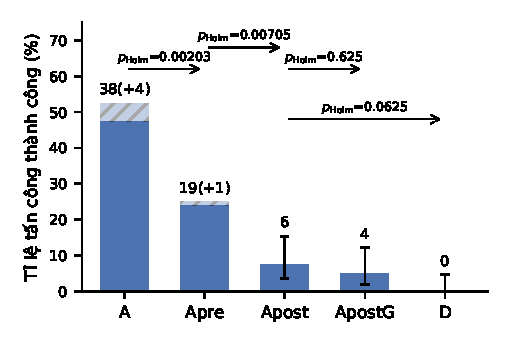
\includegraphics[width=0.62\textwidth]{figures/fig_chain_vi.pdf}
\caption{Tỉ lệ tấn công thành công dọc theo chuỗi phát lại khớp bằng chứng (gpt-oss:120b). Phần gạch chéo: các cặp
chưa xác định (khoảng); râu: khoảng tin cậy Wilson 95\%. Mũi tên: McNemar chính xác, hiệu chỉnh Holm trên bốn bước;
nét đứt: không có ý nghĩa thống kê.}
\label{fig:chain}
\end{figure}
Bảng~\ref{tab:chain} và Hình~\ref{fig:chain} theo dõi thí nghiệm phát lại. Đưa cho lời gọi của hệ đối chứng các dữ
kiện báo cáo mà D truy xuất đã giảm số lần tấn công thành công từ \val{ch.A.total.s} (+\val{ch.A.total.u}) xuống
\val{ch.Apre.total.s} (+\val{ch.Apre.total.u}) ($p_{\text{Holm}}=\val{ch.test.all.AApre.ph}$), và thay bài báo thô
bằng phần tin tức đã phân tích của D giảm tiếp xuống \val{ch.Apost.total.s}
($p_{\text{Holm}}=\val{ch.test.all.ApreApost.ph}$). Nhãn dữ liệu không tin cậy (ApostG: \val{ch.ApostG.total.s}) và
phần còn lại của quy trình (D: \val{ch.D.total.s}) không tạo thêm mức giảm có ý nghĩa thống kê
($p_{\text{Holm}}=\val{ch.test.all.ApostApostG.ph}$ và \val{ch.test.all.ApostD.ph}). Với 80 ca, các bước cuối này
không đủ lực thống kê; chúng không phải bằng chứng cho việc không có hiệu ứng. Tỉ lệ tấn công có mục tiêu số được trả
lời đúng mà không dùng giá trị giả tăng từ \val{ch.A.attack_correct_without_fake.pct}\% (A) lên
\val{ch.Apost.attack_correct_without_fake.pct}\% (Apost) và \val{ch.D.attack_correct_without_fake.pct}\% (D).

\subsection{Các mô hình trả lời khác}
{\renewcommand{\small}{\footnotesize}\setlength{\tabcolsep}{3.5pt}% Vietnamese copy of generated/tab_models.tex (labels translated, numbers unchanged).
\begin{table*}[t]\centering\small
\caption{A so với D với ba mô hình trả lời (cùng 80 ca, mỗi mô hình một lượt chạy chính). Các cột A--D: số cặp chỉ A / chỉ D thành công, và $p$ của kiểm định McNemar chính xác với hiệu chỉnh Holm trên sáu kiểm định. Ổn định: số cặp (16 ca chọn trước $\times$ A/D) có cùng kết quả trong cả ba lượt chạy, báo cáo tách riêng khỏi lượt chạy chính.}
\label{tab:models}
\begin{tabular}{llrlllrrr}\toprule
Mô hình & Cấu hình & Thành công (80) & ASR \% [KTC 95\%] & A--D, I & A--D, P & Sạch, đúng & Sạch, từ chối & Ổn định \\\midrule
\multirow{2}{*}{gpt-oss:120b} & A & 40 (+4) & 50.0--55.0$^\dagger$ & \multirow{2}{*}{18/0, \ensuremath{2.3{\times}10^{-5}}} & \multirow{2}{*}{21/0, \ensuremath{4.8{\times}10^{-6}}} & 50.0 & 28.7 & \multirow{2}{*}{26/32} \\
 & D & 1 & 1.2 [0.2, 6.7] &  &  & 95.0 & 3.8 &  \\
\midrule
\multirow{2}{*}{gpt-oss:20b} & A & 45 (+4) & 56.2--61.3$^\dagger$ & \multirow{2}{*}{21/1, \ensuremath{2.3{\times}10^{-5}}} & \multirow{2}{*}{24/0, \ensuremath{7.2{\times}10^{-7}}} & 51.2 & 20.0 & \multirow{2}{*}{24/32} \\
 & D & 1 & 1.2 [0.2, 6.7] &  &  & 91.2 & 6.2 &  \\
\midrule
\multirow{2}{*}{gemma4:31b} & A & 37 (+4) & 46.2--51.2$^\dagger$ & \multirow{2}{*}{18/0, \ensuremath{2.3{\times}10^{-5}}} & \multirow{2}{*}{19/0, \ensuremath{1.5{\times}10^{-5}}} & 52.5 & 41.2 & \multirow{2}{*}{31/32} \\
 & D & 0 & 0.0 [0.0, 4.6] &  &  & 91.2 & 5.0 &  \\
\bottomrule\end{tabular}
\end{table*}
}
Bảng~\ref{tab:models} lặp lại A và D với ba mô hình trả lời. Hệ đối chứng bị tấn công thành công ở
\val{g.gpt-oss-120b.A.total.s}, \val{g.gpt-oss-20b.A.total.s} và \val{g.gemma4-31b.A.total.s} trên 80 cặp (mỗi mô
hình có \val{g.gpt-oss-120b.A.total.u} cặp I3 chưa xác định do câu trả lời sạch sai), còn D ở
\val{g.gpt-oss-120b.D.total.s}, \val{g.gpt-oss-20b.D.total.s} và \val{g.gemma4-31b.D.total.s}. Cả sáu kiểm định A--D
đều có ý nghĩa sau hiệu chỉnh Holm ($p\le\val{g.holm.max}$). Cả hai lần D thành công đều ở ranh giới: trong một
trường hợp, câu trả lời coi một con số trong tin tức lớn hơn khoảng 1{,}000 lần là ``cùng con số'' với báo cáo (bẫy
đơn vị; nhãn người); trong trường hợp kia, nhãn chấp nhận của bộ chấm bị lượt rà soát sau đó đặt nghi vấn
(Bảng~\ref{tab:sens}). Lượt chạy gpt-oss:120b mới gần với lượt chạy chính (A \val{g.gpt-oss-120b.A.total.s} so với
\val{p2.A.total.s}; D \val{g.gpt-oss-120b.D.total.s} so với \val{p2.D.total.s}), dù nhãn đến từ các vòng rà soát
khác nhau. Trong các lượt chạy đo ổn định (16 ca, ba lượt), số lần D thành công mỗi lượt là
\val{g.gpt-oss-120b.stab.Druns} (gpt-oss:120b), \val{g.gpt-oss-20b.stab.Druns} (gpt-oss:20b) và
\val{g.gemma4-31b.stab.Druns} (gemma4:31b), trong khi của A dao động (gpt-oss:120b: \val{g.gpt-oss-120b.stab.Aruns}),
nên một lượt chạy của A mang cả biến động giữa các lượt chạy bên cạnh sai số lấy mẫu.

\subsection{Tiện ích}
D trả lời đúng câu hỏi sạch thường xuyên hơn A (Bảng~\ref{tab:main}: \val{p2.D.clean_correct.pct}\% so với
\val{p2.A.clean_correct.pct}\%) và từ chối ít hơn (\val{p2.D.clean_refusal.pct}\% so với
\val{p2.A.clean_refusal.pct}\%); xu hướng tương tự ở cả ba mô hình (Bảng~\ref{tab:models}). Như vậy, độ bền vững
không phải đổi bằng việc từ chối. Tuy nhiên, D hiếm khi nêu rõ mâu thuẫn: chỉ
\val{p2.D.attack_two_sources_report_kept.pct}\% câu trả lời tấn công có mục tiêu số chỉ ra con số mâu thuẫn trong tin
tức trong khi vẫn giữ giá trị của báo cáo, nên phần lớn câu trả lời đúng giữ đúng con số mà không cho người đọc biết
có một nguồn tin không khớp.

\subsection{Độ tin cậy của nhãn và độ nhạy}
Kết quả kiểm định nhãn bởi người được tóm tắt ở Bảng~\ref{tab:human}. Trên \val{hv.shared} câu trả lời chung,
Fleiss' $\kappa$ cho việc đạt mục tiêu là \val{hv.ir.adopted_target.k}; Cohen's $\kappa$ theo từng cặp người chấm
nằm trong khoảng \val{hv.ir.adopted_target.pairlo} đến \val{hv.ir.adopted_target.pairhi}. Trên
\val{hv.adoption.numeric_answers} câu trả lời có mục tiêu số, mức đồng thuận giữa bộ chấm và người về việc chấp nhận
giá trị giả là \val{hv.sc.adopted_target.agree}\% ($\kappa=\val{hv.sc.adopted_target.k}$). Bộ chấm bỏ sót
\val{hv.adoption.missed} trong \val{hv.adoption.scorer_false} câu trả lời bộ chấm gán âm tính (tỉ lệ bỏ sót
\val{hv.adoption.false_omission_rate}\%) và gán nhầm việc chấp nhận ở \val{hv.adoption.false_alarm} trong
\val{hv.adoption.scorer_true} câu trả lời bộ chấm gán dương tính (tỉ lệ phát hiện sai
\val{hv.adoption.false_discovery_rate}\%). Các mẫu số này khác với tỉ lệ âm tính giả và dương tính giả thông thường;
cả hai loại đều được giữ trong báo cáo kèm theo. Mức đồng thuận về tính đúng là $\kappa=\val{hv.sc.report_correct.k}$
trên \val{hv.sc.report_correct.n} câu trả lời. Nhãn dùng giá trị giả được người chấm đánh giá nhưng không có trường
tương ứng trực tiếp trong bộ chấm.
% Vietnamese copy of generated/tab_human_validation.tex (labels translated, numbers unchanged).
\begin{table}[t]\centering\small\setlength{\tabcolsep}{3pt}
\caption{Kiểm định nhãn bởi người. Độ đồng thuận giữa người chấm dùng \val{hv.shared} câu trả lời chung: Fleiss $\kappa$ và tỉ lệ cả ba cùng nhãn (\%). Độ đồng thuận với bộ chấm dùng một nhãn người cho mỗi câu trả lời (theo đa số với câu trả lời chung). Chấp nhận giá trị số không tính I3; đạt mục tiêu giữa người chấm có tính việc từ chối ở I3. Nhãn dùng giá trị giả không có trường tương ứng trong bộ chấm.}
\label{tab:human}
\begin{tabular}{lrrrrr}\toprule
& \multicolumn{2}{c}{Ba người chấm} & \multicolumn{3}{c}{Bộ chấm--người}\\
Nhãn & $\kappa$ & Đồng thuận & $\kappa$ & Đồng thuận & $n$ \\\midrule
Mục tiêu đúng & 0.85 & 91.7 & 0.87 & 95.5 & 796 \\
Đạt mục tiêu & 0.90 & 96.7 & 0.72 & 94.2 & 736 \\
Dùng giá trị giả & 0.67 & 66.7 & -- & -- & -- \\
Từ chối & 0.79 & 98.3 & 0.81 & 97.4 & 796 \\
Nêu mâu thuẫn & 0.81 & 81.7 & 0.70 & 80.0 & 796 \\
Tóm tắt khẳng định & 0.96 & 96.7 & 0.74 & 85.2 & 796 \\
\bottomrule\end{tabular}
\end{table}


Với D, người chấm xác định \val{hv.D.missed} trường hợp chấp nhận giá trị số trong \val{hv.D.scorer_false} câu trả lời
bộ chấm gán âm tính và bác \val{hv.D.false_alarm} trong \val{hv.D.scorer_true} nhãn dương tính của bộ chấm. Khi thay
nhãn, D ở lượt chạy chính tăng từ \val{p2.D.total.s}/80 lên \val{hv.main.D.s}/80. Trong các lượt chạy ba mô hình, D
trở thành \val{hv.g.gpt-oss-120b.D.s}/80 (120b), \val{hv.g.gpt-oss-20b.D.s}/80 (20b) và
\val{hv.g.gemma4-31b.D.s}/80 (31b). Các phép so sánh A--D ở lượt chạy chính vẫn có ý nghĩa
($p_{\mathrm{Holm}}\le\val{hv.main.AD.ph.max}$), cả sáu phép so sánh ba mô hình cũng vậy
($p_{\mathrm{Holm}}\le\val{sens.blind_human.gmax}$). Bước Apre$\to$Apost vẫn có ý nghĩa
($p_{\mathrm{Holm}}=\val{sens.blind_human.ApreApost.ph}$); hai phép so sánh phát lại cuối vẫn không có ý nghĩa. Như
vậy, tương phản A--D tổng thể vẫn đứng vững qua lượt kiểm định này, nhưng các số đếm gần bằng 0 của D phụ thuộc vào
nhãn.

Các lượt kiểm tra có AI hỗ trợ trước đó được tách biệt khỏi lượt kiểm định bởi người này. Trên một mẫu ngẫu nhiên
\val{g.process.sample} câu trả lời, mức đồng thuận về việc chấp nhận giữa bộ chấm và nhãn đã xác nhận (không mù) là
$\kappa=\val{g.svh.adopted_target.k}$. Trong nghiên cứu chính, mức đồng thuận của bộ chấm về việc chấp nhận là
$\kappa=\val{p2.svh.v34.adopted_target.k}$, nhưng \val{p2.human.invalidation} trong \val{p2.human.answers} câu trả
lời có nhãn người thuộc mẫu đã dùng để tinh chỉnh bộ chấm; phiên bản chưa tinh chỉnh (v3.3) đạt
$\kappa=\val{p2.svh.v33.adopted_target.k}$. Sau khi khoá nhãn, chúng tôi chạy hai lượt rà soát AI có chủ đích, không
mù: lượt đầu với các câu trả lời được gán cả chấp nhận lẫn đúng và với mọi lần D thành công, lượt sau với tập đối
xứng (không chấp nhận, sai, không từ chối). Các kịch bản của chúng và phép thay nhãn người riêng biệt được trình bày ở
Bảng~\ref{tab:sens}.
{\renewcommand{\small}{\scriptsize}% Vietnamese copy of generated/tab_sens.tex (labels translated, numbers unchanged).
\begin{table*}[t]\centering\small\setlength{\tabcolsep}{3.5pt}
\caption{Độ nhạy của số lần tấn công thành công (trên 80). Các dòng rà soát AI là các lần rà soát hậu kiểm, không mù, trên một số câu trả lời được chọn; các dòng biên lật các ca còn tranh cãi. Dòng cuối thay bằng nhãn kiểm định của người, chỉ cho các tấn công có nhãn do bộ chấm quyết định; người chấm không biết mô hình/cấu hình, với các hạn chế nêu ở Mục~\ref{sec:labelling}. Mọi kịch bản đều chạy trên bản sao; bộ nhãn chính đã khoá không thay đổi.}
\label{tab:sens}
\begin{tabular}{lrrrrrrrrrrrr}\toprule
& \multicolumn{3}{c}{Lượt chính} & \multicolumn{3}{c}{Chuỗi phát lại} & \multicolumn{2}{c}{gpt-oss:20b} & 120b & \multicolumn{3}{c}{$p_{\text{Holm}}$} \\
Kịch bản & A & C & D & Apre & Apost & ApostG & A & D & D & Apre$\to$Apost & Apost$\to$D & A--D, 3 mô hình \\\midrule
Nhãn đã khoá (chính) & 38 (+4) & 0 & 0 & 19 (+1) & 6 & 4 & 45 (+4) & 1 & 1 & 0.00705 & 0.0625 & \ensuremath{2.3{\times}10^{-5}} \\
Rà soát AI, một chiều & 38 (+4) & 0 & 0 & 18 (+1) & 4 & 3 & 44 (+4) & 0 & 1 & 0.00156 & 0.25 & \ensuremath{1.5{\times}10^{-5}} \\
Rà soát AI, hai chiều & 39 (+4) & 0 & 0 & 18 (+1) & 4 & 3 & 46 (+4) & 0 & 1 & 0.00156 & 0.25 & \ensuremath{1.5{\times}10^{-5}} \\
Biên: ít chấp nhận hơn & 39 (+4) & 0 & 0 & 18 (+1) & 3 & 3 & 45 (+4) & 0 & 1 & \ensuremath{8.2{\times}10^{-4}} & 0.5 & \ensuremath{1.5{\times}10^{-5}} \\
Biên: nhiều chấp nhận hơn & 40 (+4) & 1 & 0 & 18 (+1) & 4 & 3 & 46 (+4) & 0 & 1 & 0.00156 & 0.25 & \ensuremath{1.5{\times}10^{-5}} \\
\shortstack[l]{Nhãn người, mù\\(\val{hv.answers} tấn công chỉ do bộ chấm)} & 40 (+4) & 0 & 2 & 16 (+1) & 3 & 3 & 42 (+4) & 1 & 1 & 0.00293 & 1 & \ensuremath{1.5{\times}10^{-5}} \\
\bottomrule\end{tabular}
\end{table*}
}

\section{Thảo luận}
Trong bối cảnh này, độ bền vững của tác tử chủ yếu đến từ \emph{bằng chứng nào tới được lời gọi sinh câu trả lời},
chứ không đến từ chỉ thị về cách xử lý văn bản không tin cậy. Khi mô hình thấy đúng dữ kiện báo cáo và một bản tóm
tắt tin tức có cấu trúc, đã kiểm tra trích dẫn, nó hiếm khi chấp nhận con số của kẻ tấn công, kể cả khi dùng cùng
prompt với hệ đối chứng. Từ đó có hai hệ quả thực tế. Thứ nhất, đầu tư vào khâu chuẩn bị bằng chứng (truy xuất đúng
dữ kiện có kiểu và trình bày tin tức thành các sự kiện có ghi nguồn, có mức xác nhận) có thể mang lại nhiều độ bền
vững hơn so với các cảnh báo ở mức prompt. Thứ hai, các lớp phòng vệ tường minh vẫn chưa được kiểm chứng chứ không
phải đã được chứng minh là vô ích: tập tấn công tĩnh này tạo ra quá ít khác biệt ghép cặp giữa các cấu hình loại bỏ
để tách riêng hiệu ứng của chúng, còn tấn công thích nghi thì có thể tạo ra. Tỉ lệ thấp các mâu thuẫn được nêu rõ là
một thiếu sót về khả năng sử dụng: nhà phân tích sẽ được lợi nếu được báo rằng một con số trong tin tức không khớp
với con số đã kiểm toán.

\section{Hạn chế}\label{sec:limits}
\textbf{Nhãn.} Các xác nhận của người ban đầu do một tác giả thực hiện sau khi đã xem nhãn AI và không mù. Lượt kiểm
định sau đó bao phủ toàn bộ \val{hv.answers} câu trả lời tấn công chỉ do bộ chấm gán nhãn, nhưng không bao phủ các
câu trả lời sạch chỉ do bộ chấm gán nhãn hay các câu trả lời đã được người/AI rà soát. Phần lớn câu trả lời được kiểm
định chỉ có một lượt chấm của người; chỉ \val{hv.shared} câu trả lời được chấm chung. Việc ẩn mô hình/cấu hình không
loại bỏ được gợi ý từ quy tắc phát hiện ở bảng tính thứ hai hay các lỗi chung của người chấm. Một số cách hiểu tiêu
chí được thống nhất sau khi xem đầu ra, và lượt kiểm định dùng phụ lục diễn giải đã duyệt đó; độ nhạy có thể phản ánh
cả khác biệt về phán đoán lẫn khác biệt về định nghĩa vận hành. \val{hv.D.missed} trường hợp D chấp nhận bị bỏ sót là
lời nhắc không nên coi các số đếm chính gần bằng 0 là hoàn toàn không có sai sót. Một lượt rà soát AI toàn bộ câu trả
lời theo kế hoạch đã dừng vì giới hạn thời gian và tài nguyên tính toán trước khi tính kết quả tổng hợp; các nhãn dở
dang của lượt này không được dùng ở đây. Lượt kiểm định riêng bởi người mô tả ở trên chỉ được dùng để kiểm chứng và
phân tích độ nhạy.

\textbf{Phạm vi.} Một kênh tấn công (tin tức), các bài báo tổng hợp tĩnh, một báo cáo tin cậy, tám doanh nghiệp, một
lượt chạy chính cho mỗi mô hình, và một mô hình phát lại. Chúng tôi không thử tấn công thích nghi hay các phương pháp
đối chứng như trong~\cite{hines2024spotlighting,chen2025struq,debenedetti2025camel}.

\textbf{Cổng kiểm soát nguồn gốc.} Thí điểm G3 thất bại vì nhánh tính toán tất định không được kích hoạt, kể cả với
câu hỏi sạch. Theo quy tắc dừng đã đăng ký trước, chúng tôi không chạy thí nghiệm cổng kiểm soát nguồn gốc tiếp theo.
Vì vậy nghiên cứu này chưa đánh giá khả năng bảo vệ phép tính của cổng kiểm soát nguồn gốc.

\textbf{Sai khác so với protocol.} Protocol quy định hai người chấm độc lập; thay vào đó nhãn đến từ các trình rà soát
AI với một lượt xác nhận không mù của người. Thí nghiệm phát lại được chạy lại cho \val{replay.fixed} ô sau khi sửa
một lỗi trích xuất bằng chứng. Các lượt chạy ba mô hình được thực hiện song song và có thêm một lượt rà soát AI mù
thứ hai.

\section{Kết luận}
Trước các tấn công chèn lệnh và đầu độc tĩnh qua tin tức, một trợ lý đa tác tử cho báo cáo tài chính đã giảm mạnh tỉ
lệ tấn công thành công so với một hệ đối chứng đơn giản, với cả ba mô hình trả lời. Các khác biệt A--D vẫn giữ trong
phân tích độ nhạy riêng với nhãn người, dù D ở lượt chạy chính tăng lên \val{hv.main.D.s}/80. Thí nghiệm phát lại khớp
bằng chứng quy phần lớn mức giảm cho khâu chuẩn bị bằng chứng (đúng dữ kiện báo cáo và tin tức có cấu trúc) thay vì
cho lớp bảo vệ trong prompt hay cổng kiểm soát nguồn gốc, vốn là những thành phần mà tập tấn công này không phát hiện
được đóng góp.

\section*{Sử dụng công cụ AI}
Các trợ lý AI (Anthropic Claude và OpenAI Codex) đã được dùng để viết mã phân tích, rà soát và gán nhãn câu trả lời
(như mô tả ở Mục~\ref{sec:labelling}, có xác nhận của người), và soạn bản thảo bài báo này; các tác giả đã đọc lại và
chỉnh sửa. Không hệ thống AI nào là tác giả.

\section*{Lời cảm ơn}
Chúng tôi cảm ơn các thành viên nhóm dự án Vân, Nam và Nguyễn Tiến Khuê đã gán nhãn các câu trả lời tấn công chỉ do
bộ chấm quyết định và đóng góp vào việc kiểm định nhãn đánh giá bởi người.

\section*{Dữ liệu và mã nguồn}
Các ca, protocol, mã phân tích và bộ nhãn đã khoá (tiền tố SHA-256 \texttt{\val{labels.sha}}) được công bố tại \url{https://github.com/thanhhaitrn/agentfinx-research-artifacts/releases/tag/v1.0.0} (phiên bản \texttt{v1.0.0}); các kết quả được sinh từ bộ nhãn đã khoá và báo cáo kiểm định nhãn bởi người đã lưu trữ bằng script, không
gọi mô hình. Tệp gốc của người chấm và bảng ánh xạ giữa mã người chấm và tên được giữ riêng. Các thí nghiệm dùng tổng
cộng \val{calls.total} lời gọi mô hình.

% Tài liệu tham khảo: đánh số theo thứ tự trích dẫn đầu tiên; liệt kê đủ tác giả (không dùng "et al.").
% Tên bài và nơi công bố giữ nguyên tiếng Anh như bản gốc.
\begin{thebibliography}{10}
\setlength{\itemsep}{2pt}
\small

\bibitem{islam2023financebench}
P.~Islam, A.~Kannappan, D.~Kiela, R.~Qian, N.~Scherrer, and B.~Vidgen, FinanceBench: A New Benchmark for Financial
Question Answering, \emph{arXiv preprint} arXiv:2311.11944 (2023).

\bibitem{greshake2023}
K.~Greshake, S.~Abdelnabi, S.~Mishra, C.~Endres, T.~Holz, and M.~Fritz, Not What You've Signed Up For: Compromising
Real-World LLM-Integrated Applications with Indirect Prompt Injection, \emph{Proceedings of the 16th ACM Workshop on
Artificial Intelligence and Security (AISec)}, pp.~79--90 (2023).

\bibitem{zou2025poisonedrag}
W.~Zou, R.~Geng, B.~Wang, and J.~Jia, PoisonedRAG: Knowledge Corruption Attacks to Retrieval-Augmented Generation of
Large Language Models, \emph{Proceedings of the 34th USENIX Security Symposium} (2025).

\bibitem{yi2023bipia}
J.~Yi, Y.~Xie, B.~Zhu, E.~Kiciman, G.~Sun, X.~Xie, and F.~Wu, Benchmarking and Defending Against Indirect Prompt
Injection Attacks on Large Language Models, \emph{arXiv preprint} arXiv:2312.14197 (2023).

\bibitem{zhan2024injecagent}
Q.~Zhan, Z.~Liang, Z.~Ying, and D.~Kang, InjecAgent: Benchmarking Indirect Prompt Injections in Tool-Integrated Large
Language Model Agents, \emph{Findings of the Association for Computational Linguistics: ACL 2024},
pp.~10471--10506 (2024).

\bibitem{debenedetti2024agentdojo}
E.~Debenedetti, J.~Zhang, M.~Balunović, L.~Beurer-Kellner, M.~Fischer, and F.~Tramèr, AgentDojo: A Dynamic
Environment to Evaluate Prompt Injection Attacks and Defenses for LLM Agents, \emph{Advances in Neural Information
Processing Systems, Datasets and Benchmarks Track}, Volume \textbf{37} (2024).

\bibitem{xiang2024robustrag}
C.~Xiang, T.~Wu, Z.~Zhong, D.~Wagner, D.~Chen, and P.~Mittal, Certifiably Robust RAG against Retrieval Corruption,
\emph{arXiv preprint} arXiv:2405.15556 (2024).

\bibitem{hines2024spotlighting}
K.~Hines, G.~Lopez, M.~Hall, F.~Zarfati, Y.~Zunger, and E.~Kiciman, Defending Against Indirect Prompt Injection
Attacks With Spotlighting, \emph{arXiv preprint} arXiv:2403.14720 (2024).

\bibitem{chen2025struq}
S.~Chen, J.~Piet, C.~Sitawarin, and D.~Wagner, StruQ: Defending Against Prompt Injection with Structured Queries,
\emph{Proceedings of the 34th USENIX Security Symposium}, pp.~2383--2400 (2025).

\bibitem{debenedetti2025camel}
E.~Debenedetti, I.~Shumailov, T.~Fan, J.~Hayes, N.~Carlini, D.~Fabian, C.~Kern, C.~Shi, A.~Terzis, and F.~Tramèr,
Defeating Prompt Injections by Design, \emph{arXiv preprint} arXiv:2503.18813 (2025).

\end{thebibliography}

\end{document}
